\chapter{Octree- \&
Voxel-driven Exploration}\label{chap:3:title}
% \chapter{Method}\label{chap:3:title}

\begin{figure}[!ht]
        \centering
        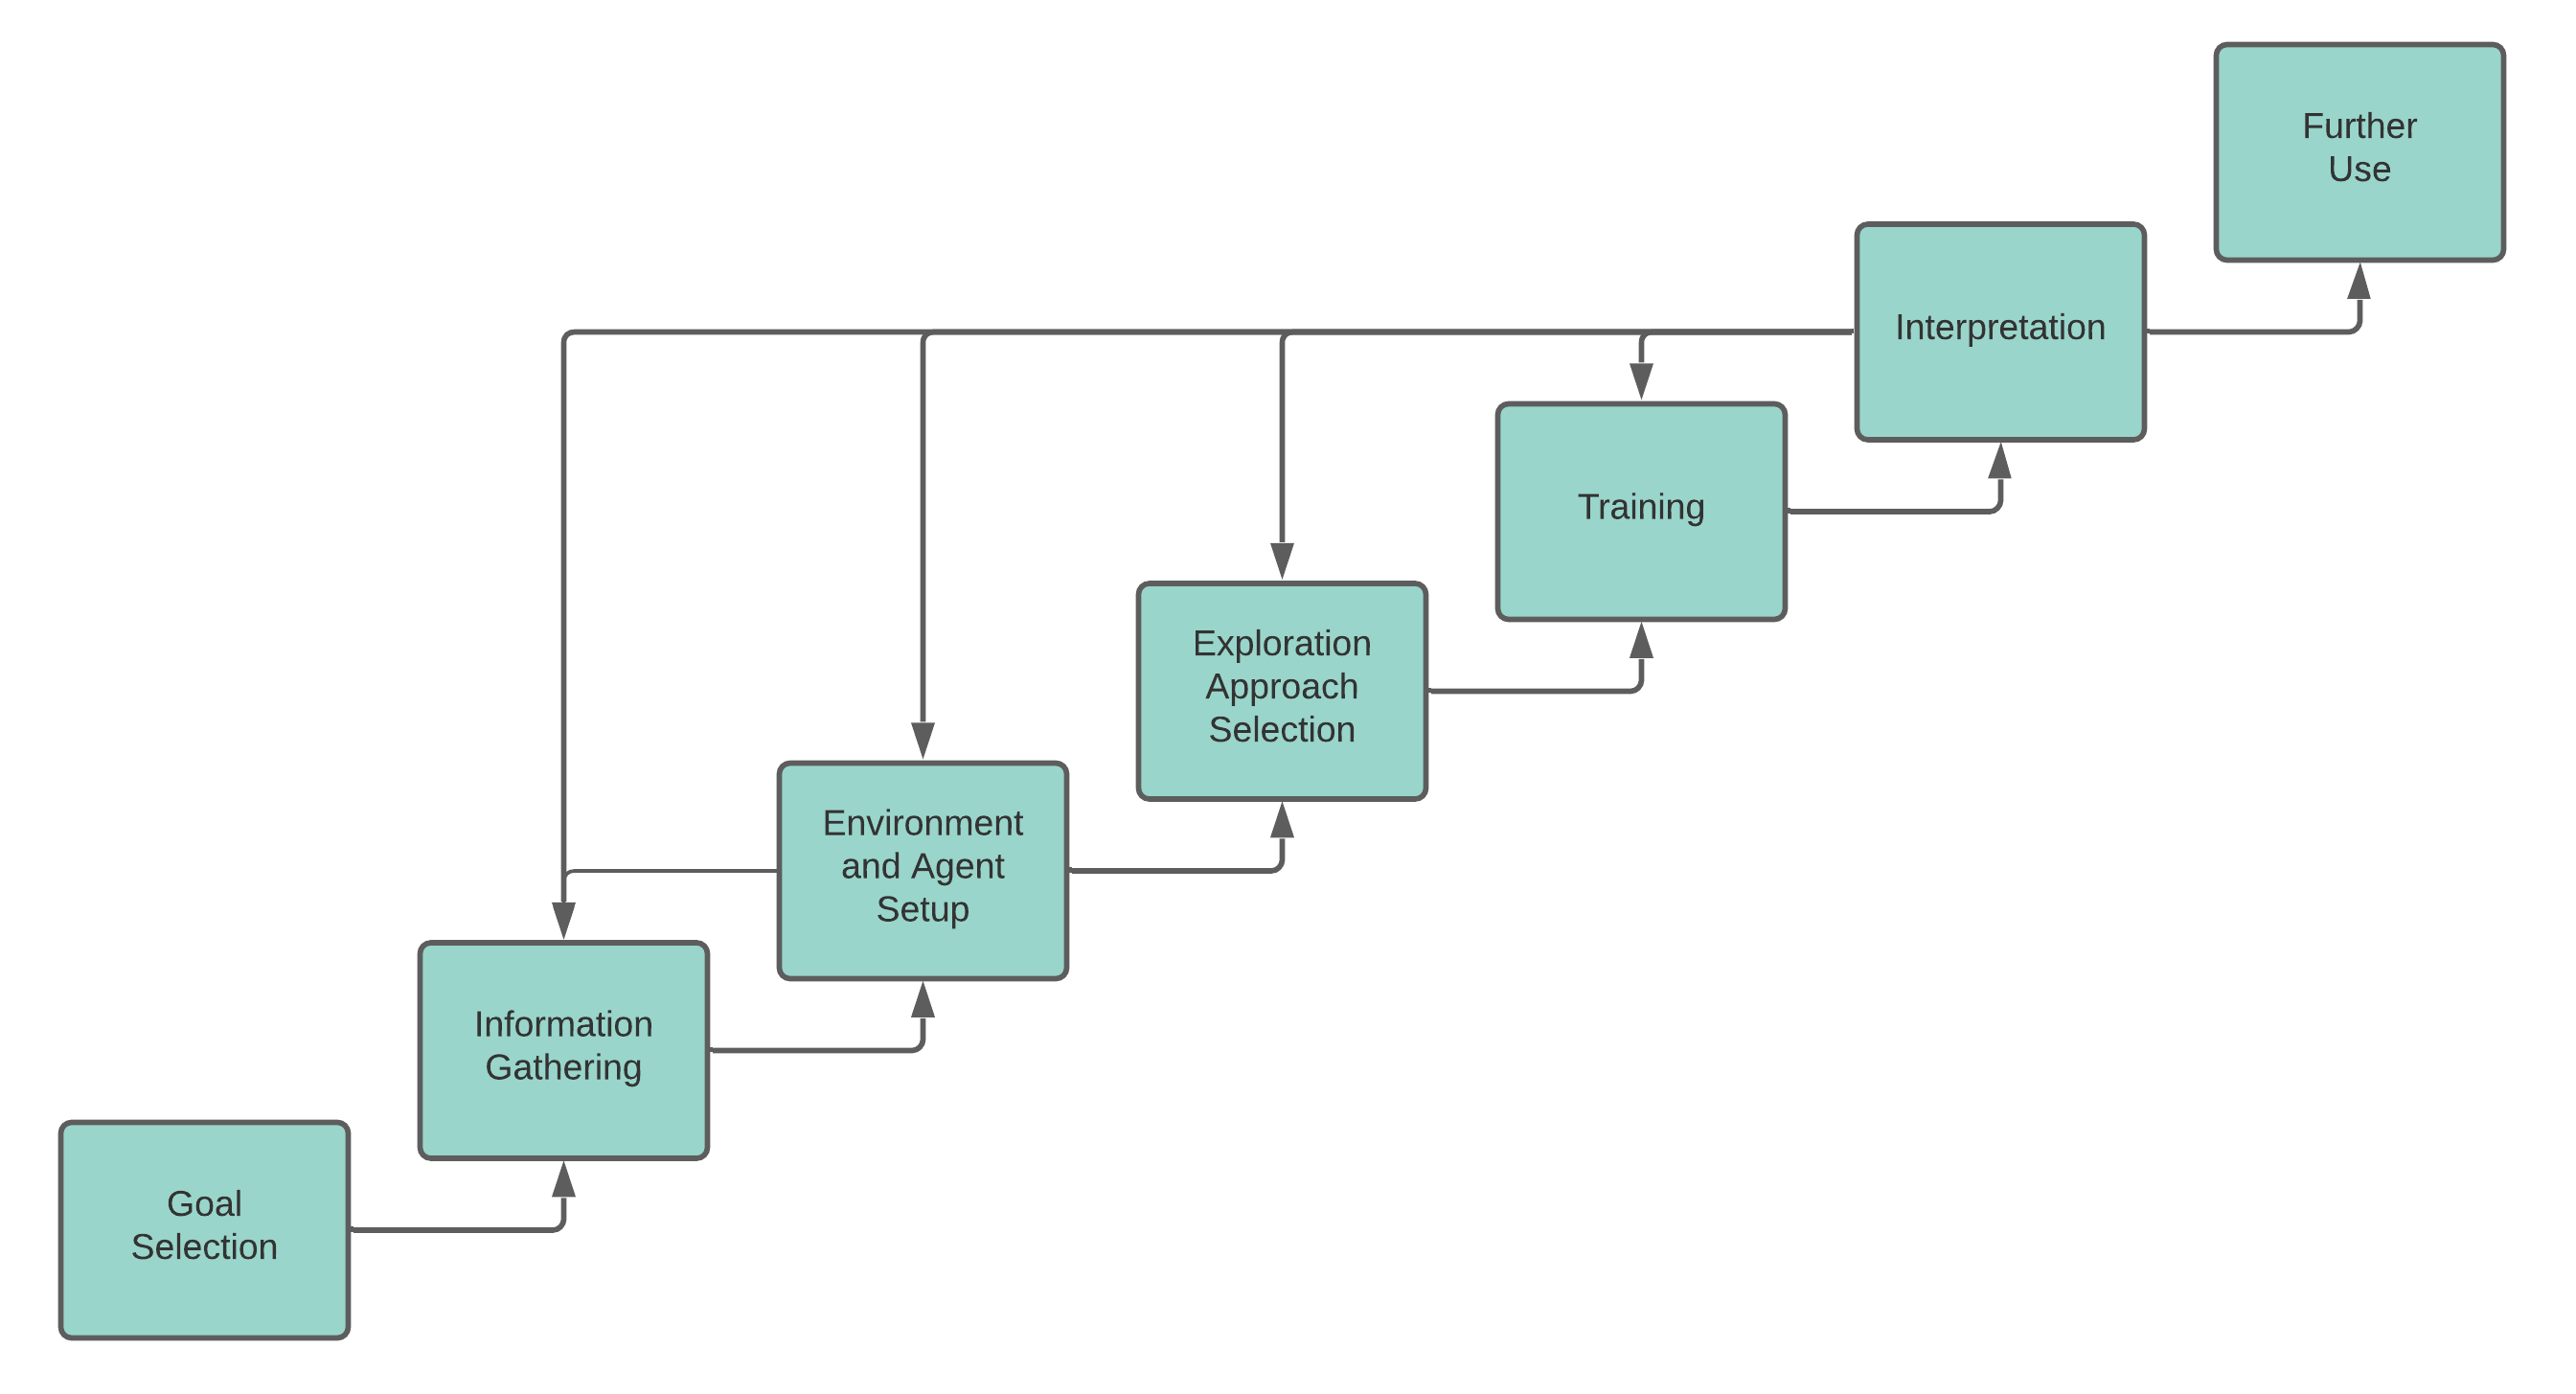
\includegraphics[width=1\textwidth]{images/adapted_development_process_exploration_v2.png}
        \caption{Adapted development process from "\citetitle{luckert2016using}", by \textcite{luckert2016using}. Describes the taken steps from data collection, through algorithm selection to architecture design.}
        \label{fig:development_design}
\end{figure}
In this chapter, the different steps taken to construct the environment and the reinforcement learning agent are addressed. 
This chapter adapts the structure proposed for machine learning algorithms proposed by \textcite{luckert2016using}.
The following questions are answered during this chapter:
\begin{itemize}
    % \item What kind of data is necessary?
    % \item What is the process for modeling 3D environments for exploration?
    % \item What are the 
    \item What are the current method's goals and limits?
    \item How was the reinforcement learning environment modeled and set up?
    % \item How was the agents perception defined?
    \item How is the agent-observable data constructed?
    % \item How are voxels generated from RGBD data?
    % \item What is Unity ML Agents for reinforcement learning?
    \item How was the agent's character defined (3D model, movement, etc.)?
    \item What reinforcement learning approach was chosen? 
    \item How is the proposed method composed? 
    % what method (of all the compared ones) provides the possibility to answer the research questioon and how is it composed? ....
    % \item What is the method's pipeline composed of?
    % \item What attributes apply to the learning agent?
    \item How can the proposed exploration method be further applied?
\end{itemize}


In order to answer these questions, the structure of this chapter is illustrated in Figure \ref{fig:development_design}.
The first step of the RL process is discussed in Section \ref{chap:3:goal}, which defines the exploration task and limits its scope. 
Then, the choice of a suitable 3D environment for exploration where the agent collects observations from (i.e., the data set) and the construction of the 3D environment is presented. 
% collected raw data as
Section \ref{chap:3:data} introduces the modeling process and setup of the 3D environment.
% /the 3D assets, components and variables that compose the environment.
% information available (voxels, octree data) and the choice of observations for the given task
Afterwards, it explains the approach to perception, presenting the process of voxelization, the creation of the octree map.
% , the grid sensor component and the concept of semantic entropy.
Then, it outlines the sensors used in the agent for visual input and the usage of semantic entropy to define uncertainty in an environment.
% 
% preprocessing of the data by identifying noise or erroneous inputs. 
% preesents the choiceof three proposed processing pipelines and the considered algorithms and techniques. T
The agent's character, including 3D models, movement algorithms and other components are presented in Section \ref{}.
Furthermore, the choice of agent observations, reward signal and environment-related behaviors are defined in Section \ref{chap:3:agent-choice-actions} and the description of the chosen reinforcement learning algorithm is covered in Section \ref{chap:3:specification-approach}. Subsequently, the interpretation of the exploration approaches to octress and voxels are described in Section \ref{chap:3:interpretation}. 
This section also tackles how the method's performance was measured and evaluated and which parameters were tuned.
% the algorithms were compared to each other
Finally, Section \ref{chap:3:further-use} presents the proposed evaluation framework for the assessment and comparison of the learned behaviors, introduces the applicability of our approach in multiple scenarios, presents the transferability of the learning environment to another environment platform and proposes the comparison of the performance of the PPO with the Soft Actor-Critic algorithm for the given setup.
% for the experiments to evaluate and compare learned behaviors.
% dacross for determining the 3D position of the salient object. 
% It also sets out the assumptions we took and the choices of technologies with respect to what was discussed in Section 2.
Inspired by the structure proposed by \textcite{luckert2016using} and given the iterative nature of the reinforcement learning process, this work was split into two main loops:
\begin{itemize}
    \item The first loop includes steps 2 and 3, and involves the groundwork for the learning algorithm: it involves the manual construction of the learning environment and the agent using Unity \cite{unity2021} for fabricating the 3D scenes and the ML-Agents SDK \cite{github-unity-mlagents-toolkit}. This resulted in a high dependency between the 3D modeling, the simulation of a real robot and the  abstractions provided by the learning platform, which demanded an iterative development process.
    
    \item The second loop includes steps 2-6, which allows the readjustment of 3D models, the learning environment, agent attributes, observations, reward signals, step size, voxel models, octree parameters, entropy definition, etc. This loop is critical for this thesis, since the main objective is the optimization of exploration strategies for unknown environments. For this purpose, the presented iterative process was used and multiple baselines were proposed to provide performance comparisons. Furthermore, the diverse algorithms performance can be inspected in real-time in Unity and therefore require readjustments in steps 2 and 3.

    % can be explained through the working loop illustrated in Figure \ref{development_design}. This loop allows the 
\end{itemize}

% domain model
%  
\section{Identification of Goals}\label{chap:3:goal}
The predetermined goal of this project work was to propose an exploration policy that reduces uncertainty in a 3D scene. As mentioned in Section \ref{chap:1:research-question}, this project work tackles the following research questions: 
\begin{itemize}
    %  Howcan an active vision exploration policy based on a ubiquitous source of information such as voxels, in currently accessible RGBD cameras, contribute to reducing the uncertainty about a scene?
     % \item How can these exploration policies be leveraged for a multitude of scenarios, including the milking robot problem? 
   
    % \item How can 3D data (meshes or point clouds), in voxel form, be exploited for extrinsic motivation for the exploration of objects in an unknown environment?
    % \item How can large and unknown environments be explored efficiently by the same agent?
    % \item How can uncertainty be defined through semantic entropy and be used as a motivation in exploration policies?
    \item How can an embodied agent increase the overall certainty about an object's characteristics, i.e., how can trajectories around objects of interest be generated to reduce the uncertainty about such objects? 
    \item How can these objects be found in large and unknown environments by the same agent?
    
   
  
    
\end{itemize}

% \begin{itemize}
%     \item How can the cow teats 3D pose be estimated under 10 seconds?
%     % \item How can the cow teats 3D pose and direction estimation be evaluated?
% \end{itemize}
To answer these questions, the following practical steps were laid out:
\begin{enumerate}
    \item Model and present a 3D environment for a learning agent to explore and find objects of interest.
    \item Define the perception approach for the agent and the character baseline, which includes 3D models, movement algorithms, sensors and limitations.
    % \item Define the perception approach, specifying how the agent sees in such environments.
    % \item Define the learning agent's baseline, specifying the 3D models, movement algorithms and other components.
    \item Choose and describe the reinforcement learning approaches for two goals: a) exploration of an environment and b) exploration of objects.
    % , including the reinforcement learning algorithm to achieve such behaviors.
    % by constructing an octree with the agent's trajectory and scan radius. 
    % \item Define the reinforcement learning approach, which includes the choice of observations, goal and reward signal and implementation.
    \item Propose learning variants based on the influence of different observations and reward alternatives.
    % \item Present the further use of results, comprised of an evaluation framework, goal scenarios, cross-platform performance and algorithmic performance. 
    % vision processing pipeline with optimal prediction quality for identifying the 3D pose and direction of a cow teat.
    % \item Present a method for evaluating the quality of the predictions regardless of the method used.
\end{enumerate}
This strategy was determined because the steps for the 3D modeling of environments are independent of the reinforcement learning approach used. Therefore, the remaining task is to propose a reinforcement-learning-enabled pipeline that aims to solve the indicated exploration task without a priori knowledge of a 3D environment.
% knowledge of the input system, is the usage of the diverse types of information the 
The main challenge in the exploration pipeline lies in the choice of the diverse types of observations the environment can provide to the agent. The diverse variants of the reinforcement learning algorithm will then be built on the outcome of the second step.
Therefore, the definition of the environment, the goals and the agent's capabilities focuses on the working steps 1 and 2. The remaining steps are solved by using the modeled environments and the agent character. 
More concretely, the population of an octree through the agent's trajectory to solve the exploration task concentrates on the third working step. This working step also includes the exploration of objects, for which the voxelization of 3D meshes is chosen as an efficient and thorough representation of the agent's goals. We call this interest to explore goals through voxels "voxel curiosity".

Additionally, we define uninformativeness in an environment and around the objects is not only by the states that are new to the agent, but also through \textit{semantic entropy}. This concept is inspired by research in semantic curiosity \cite{chaplot2020semantic} and is addressed in the second working step, as uninformativeness is not only given by the modernity of a state $s$ but also through the temporal class density in such state.
% , while the  is tackled on the third working step. 
Finally, in the last working step, the further use of results is presented, including the influence of the observations and rewards in the exploration policies.
% are presented as a result of combining the different observations and rewards available to the agent, which allows the measurement of the influence of each observation in the agent's performance.

% The method for evaluating the quality of the predictions will then be built on the results of the processing pipeline. Therefore, the computer vision task is solved by the first step and and the second one is solved by looking at the prediction outputs.
An important limitation, as mentioned in section \ref{chap:1:scope}, is that this work focuses on reinforcement-learning-based exploration of an environment through ubiquitous visual information (voxels) to reduce uncertainty (defined through entropy) and does not take data sampling in the agent's trajectories or integration of further semantic modules into account, since this would go beyond the scope of this thesis.

\section{Specification of the Learning Environment}\label{chap:3:data}
% Reinforcement Learning Data
% computer vision predictions it is essential to gather sufficient quantities of raw data and to layout a simple data structure 
Data in a reinforcement learning problem is obtained through the environment and the diverse states the agent traverses. Therefore, in order to train and evaluate the agent, it is essential to define a 3D scene which provides information to the agent and delimits the exploration problem.
% the information visible to agent, etc., as required. 
The following questions will be answered in this section:
\begin{itemize}
    % \item What kind of data is necessary?
    % \item What kind of structure fulfills the requirements for the present study?
    % \item What is the origin of the data?
    % \item What are the preprocessing steps?
    \item What led to choosing Unity 3D as the preferred 3D modelling and simulation engine?
    \item What led to choosing \textit{Unity ML-Agents} as the preferred environment platform?
    % \item What led to using Unity 3D for this work?
    % \item How was the environment modelled in Unity 3D?
    % % \item How was the agent set up?
    
    % could be moved to next section
    % \item How are voxels generated?
    % \item How are the nodes in the octree constructed?    
    % \item How is visual uncertainty in an environment defined through semantic entropy?
    % \item How is semantic entropy measured?
\end{itemize}

Training a reinforcement learning agent requires the following: 1) a learning environment, 2) an agent that can observe the environment and choose actions in such environment; 3) a learning algorithm appropriate for the states present in the environment (continuous, discrete). 
% Traditional computer vision tasks require the following types of data: a training data set, for training the algorithm on the domain-specific data and a test set to determine the algorithm's prediction quality. 
As stated in Section \ref{chap:3:goal}, the given task is to explore an unknown environment while reducing uncertainty in the environment itself and the objects in it. Therefore, the agent requires: 1) motivation to navigate and explore the environment, 2) motivation to investigate objects exhaustively, and 3) a way to take into account if there is uncertainty or "uninformativeness" while it is exploring. This last requirement is defined through semantic entropy in subsection \ref{chap:3:semantic-entropy}. 
% The following subsections present the approach chosen to solve such task.
The following sections presents the 3D scene and the steps required to construct the environment states for the agent.
% and the underlying logic required for posterior learning

\subsection{A Unity 3D Environment}
The first step requires setting up the environment for the agent. The best game engines in the market right now are Unity 3D and Unreal Engine 4. Both engines allow exhaustive development of gaming environments, with support for scripting languages, and a considerable toolset for animations, triggers, physics simulations, etc. However, Unity was the engine chosen for the setup of this work given its simpler interface, bigger community, and its state-of-the-art plugin for reinforcement learning
Unity \textit{ML-Agents} \cite{incredibuild2021unityvsunreal, juliani2018unity}. 
For more information on the 3D modelling using Unity 3D, please refer to Appendix \ref{appendix:unity3d-environment-modeling}.


\begin{figure}[!ht]
        \centering
        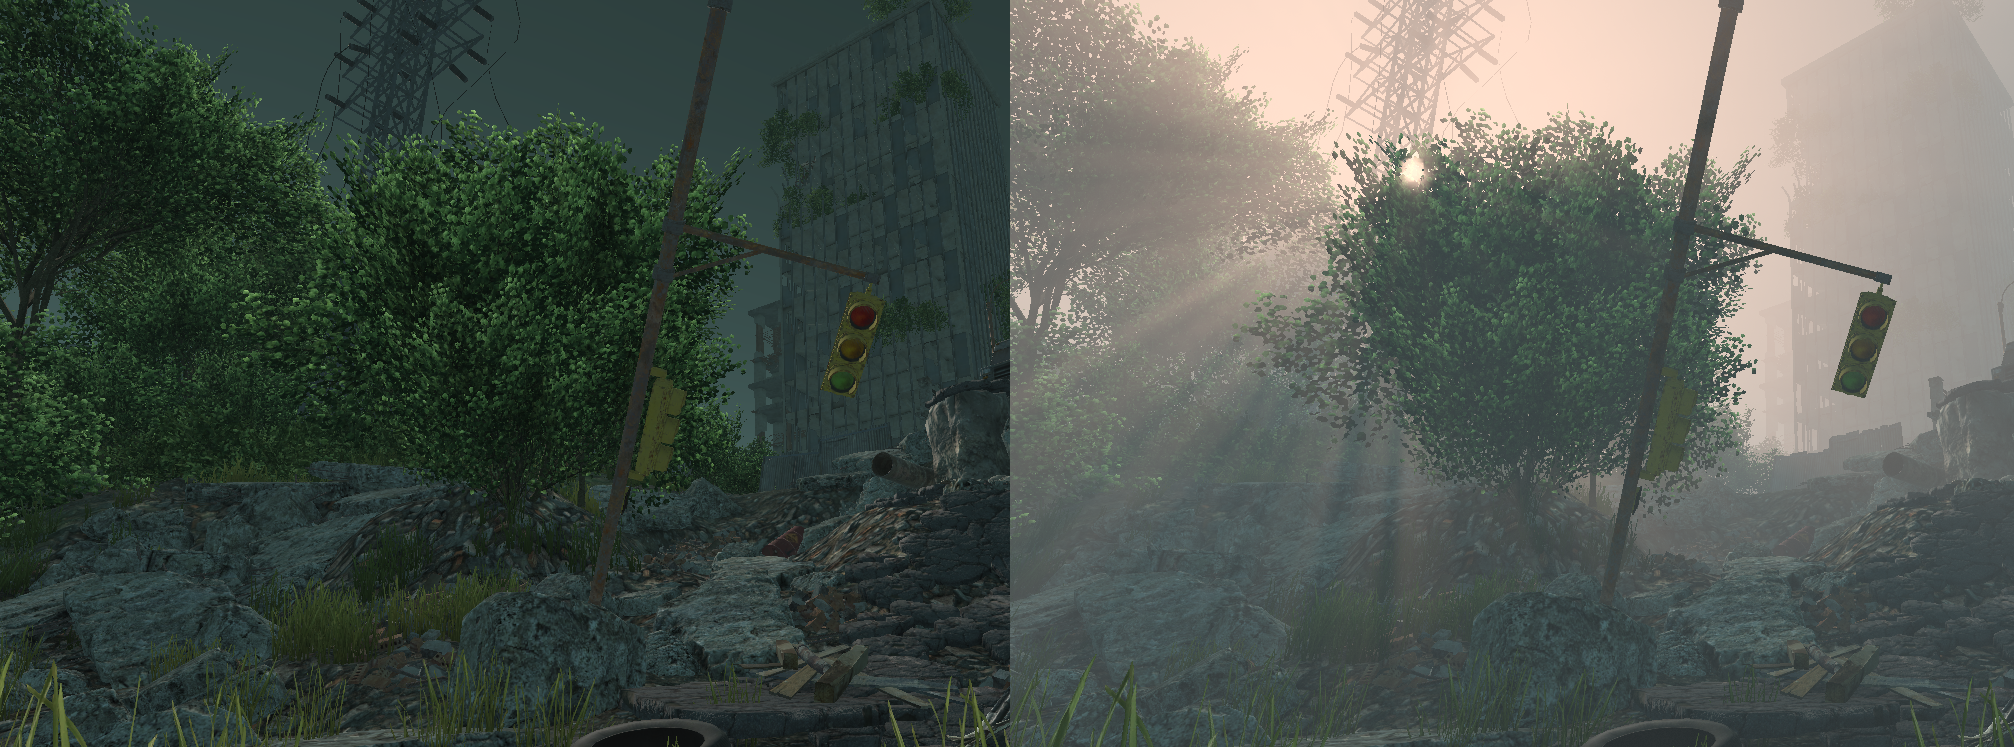
\includegraphics[width=0.8\textwidth]{images/unity-lighting.png}
        \caption{Example of a 3D scene without lighting settings (left) and the same scene with post-processing effects (right). Factors like depth, high-quality volumetric light and fog of variable density allow the construction of realistic environments. Taken from \cite{unity_volumetric_light}.
        }
        \label{fig:unity-light}
\end{figure}

In the setup of a scene, a variety of environment assets such as buildings, trees, rocks, and foliage, are required to convey an authentic depiction of a scene. Sample screenshots of these assets, as well as of the visual effects and skybox assets are illustrated in appendix Figure \ref{fig:assets-unity}. Once all the assets are allocated in a scene, the rendering pipeline can be tuned to adjust the lighting settings to achieve a more realistic rendering if needed. Figure \ref{fig:unity-light} shows the difference lighting makes when simulating a 3D scene, which is one of the many parameters, in addition to color, texture, rotation, position, etc., that can be randomized using a game engine. 
As mentioned in Section \ref{chap2:synthetic-data}, domain randomization allows the creation of a dataset that includes not only corner cases but also allows the learning algorithm to generalize to unseen environments.


Given that the current approach utilizes a grid sensor, octrees and voxels to abstract the 3D environment, the realism of the scene does not play a role in the agent's performance. This setup allows the separation of the 3D modeling work from the agent's algorithm, while still being able to extend to other use cases that can exploit Unity's scripting framework and domain randomization capabilities.



\subsection{Environment Platforms}
An environment platform enables the development, training, and testing of reinforcement learning algorithms. It also provides the necessary interfaces to abstract the interaction between the logic running on a system and the environment that the agent is interacting with.
More concretely, the environment platform provides a variety of features that allow the definition of the state of the game, the actions the agent can perform, the reward functions, and the training strategy. We introduce two environment platforms in the following sections: OpenAI Gym and Unity ML-Agents.

\subsubsection{OpenAI Gym}
OpenAI Gym \cite{github-unity-mlagents-toolkit} is a platform designed to facilitate the development of reinforcement learning agents. OpenAI Gym has been integrated into several popular reinforcement learning systems, including the open-source reinforcement learning platform OpenAI Baselines. Gym supports both training and test modes with a variety of configurations to evaluate and compare algorithms, unifying researchers in reinforcement learning to a common set of interfaces, and abstracts the environment through the \textbf{env} interface. This interface provides the following main abstractions:
\begin{itemize}
    \item \textbf{reset(self).} This resets the environment and returns an observation.
    \item \textbf{step(self, action).} Transitions the environment to state $s_{t+1}$ and returns a tuple of type: \textit{(observation, reward, done, info)}.
    \item \textbf{render(self).} Renders the environment in its current timestep.
\end{itemize}

\subsubsection{Unity ML-Agents}
Unity ML-Agents \cite{github-unity-mlagents-toolkit} is an RL platform which allows the construction of more environments rich in physical and sensory complexity, leveraging the Unity game engine, which is composed of a set of components that enable physics simulations, realistic renderings, etc., as described in Section \ref{chap2:3denvironment}. The platform not only 
provides an abstraction layer for the development of algorithms and sophisticated tasks like autonomous driving, but also supports the development of complex multi-agent applications, curriculum learning, imitation learning, etc \cite{github-unity-mlagents-toolkit}. This is also facilitated given their state-of-the art implementations of algorithms to easily train agents for 2D, 3D, and VR / AR applications. In contrast to OpenAI gym, the ML-Agents toolkit is composed of the following components, illustrated in Figure \ref{fig:unity-learning-environment-full}:

\begin{itemize}
    \item \textbf{Learning Environment.} It encapsules the Unity scene and \textit{game characters}. The Unity scene sets up the environment for the agent to observe, act and learn and has to be modeled and constructed by the developer. The ML-Agents plugin allows the transformation of the scene into a reinforcement learning environment. It uses the Academy component (not illustrated) to ensure that all \textit{Agents} are synchronized and to manage the learning environment's settings.
    % The learning environment through the Academy (not represented in the diagram) ensures that all the Agents are in sync in addition to controlling environment-wide settings.

    % which contains the Unity scene and all the game characters. The Unity scene provides the environment in which agents observe, act, and learn. How you set up the Unity scene to serve as a learning environment really depends on your goal. You may be trying to solve a specific reinforcement learning problem of limited scope, in which case you can use the same scene for both training and for testing trained agents. Or, you may be training agents to operate in a complex game or simulation. In this case, it might be more efficient and practical to create a purpose-built training scene. The ML-Agents Toolkit includes an ML-Agents Unity SDK (com.unity.ml-agents package) that enables you to transform any Unity scene into a learning environment by defining the agents and their behaviors.
    % 
    \item \textbf{Python Low-Level API.}. This is the low-level Python interface which allows communication with a learning environment. This component is separate from Unity, in contrast to the learning environment, and uses the Communicator to interact with the Unity environment.
    
    % which contains a low-level Python interface for interacting and manipulating a learning environment. 
    % Note that, unlike the learning environment, the Python API is not part of Unity, but lives outside and communicates with Unity through the Communicator. 
    % This API is contained in a dedicated mlagents\_envs Python package and is used by the Python training process to communicate with and control the Academy during training. 
    % However, it can be used for other purposes as well. For example, you could use the API to use Unity as the simulation engine for your own machine learning algorithms. See Python API for more information.
    \item \textbf{External Communicator.} This component enables the interaction between the learning environment and the Python Low-Level API.
    % which connects the learning environment with the Python Low-Level API. It lives within the learning environment.
    \item \textbf{Python Trainers.} The trainers contain the machine learning algorithms that realize reinforcement learning. They are implemented in Python and interface through the Python Low-Level API.
    % which contains all the machine learning algorithms that enable training agents. The algorithms are implemented in Python and are part of their own mlagents Python package. The package exposes a single command-line utility mlagents-learn that supports all the training methods and options outlined in this document. The Python Trainers interface solely with the Python Low-Level API.
    \item \textbf{Gym Wrapper.} This component allows the export of learning environments to an OpenAI Gym \cite{github-openai-gym} environment platform. OpenAI Gym is a common platform for developing and comparing reinforcement learning algorithms. 
    % enabling the usage of many different architectures and set ups for training agents. 
    This component is not illustrated. 
    % A common way in which machine learning researchers interact with simulation environments is via a wrapper provided by OpenAI called gym. We provide a gym wrapper in a dedicated gym-unity Python package and instructions for using it with existing machine learning algorithms which utilize gym.

\end{itemize}

\begin{figure}[!ht]
        \centering
        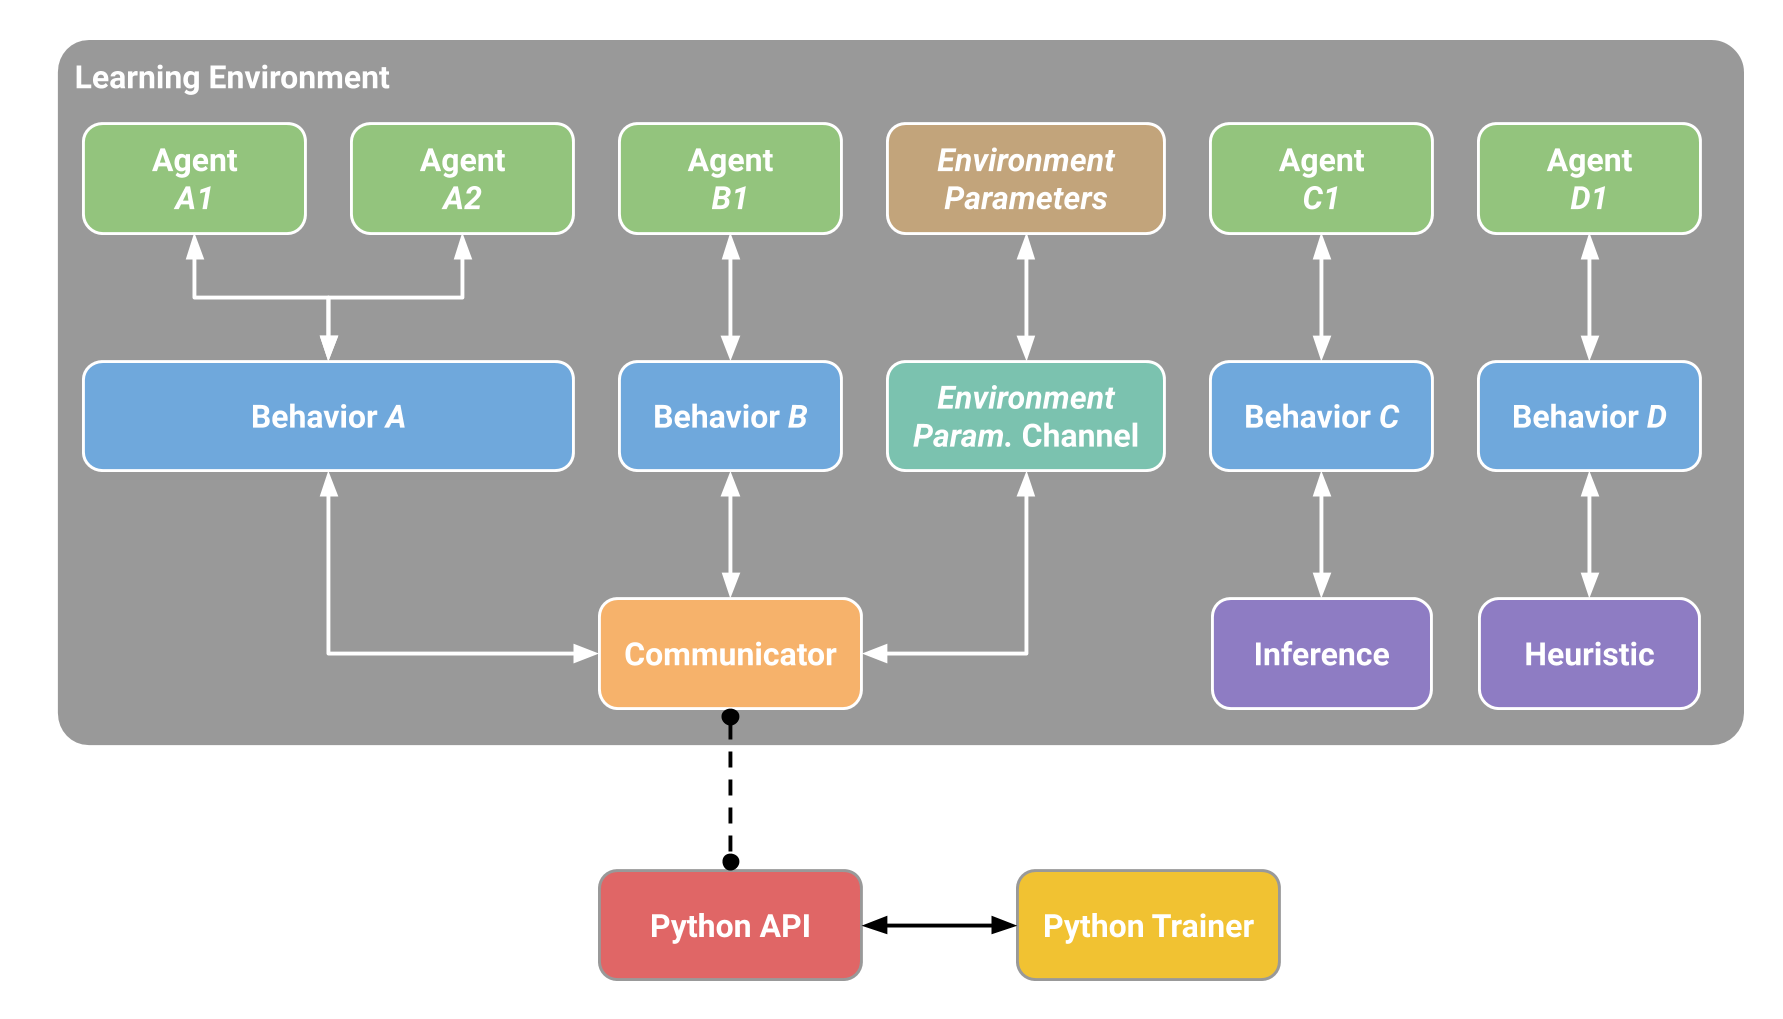
\includegraphics[width=0.96\textwidth]{images/unity-learning_environment_full.png}
        \caption{Overview of the Unity ML-Agents Toolkit, taken from \cite{github-unity-mlagents-toolkit}.
        }
        \label{fig:unity-learning-environment-full}
\end{figure}


Accordingly, the following components in the learning environment aid in the organization of the Unity scene: 
% learning environment
% The learning environment contains two Unity Components that help organize the Unity scene:
\begin{itemize}
    \item \textbf{Agents.} This component abstracts the provision of observations, execution of actions and assignment of rewards and penalties.
    It is attached to a Unity GameObject, which can be any character in the scene, and is linked to a \textit{Behavior}.
    % which is attached to a Unity GameObject (any character within a scene) and handles generating its observations, performing the actions it receives and assigning a reward (positive / negative) when appropriate. Each Agent is linked to a Behavior.
    \item \textbf{Behavior.}. A Behavior component is the logic that takes observations and rewards and returns actions to execute. 
    It also defines the essential characteristics of an agent, such as the type and number of actions the agent can take.
    Finally, it can be of three types: a) a \textit{learning behavior} that communicates that a model should be created and activates the learning process, b) a \textit{heuristic behavior} that limits itself to a set of hard-coded rules for the agent movement, or c) an \textit{inference behavior} that loads a selected learned model and executes the learned policy in the learning environment.
    
    % of the agent.
    % - defines specific attributes of the agent such as the number of actions that agent can take. Each Behavior is uniquely identified by a Behavior Name field. A Behavior can be thought as a function that receives observations and rewards from the Agent and returns actions. 
    
    % A Behavior can be of one of three types: Learning, Heuristic or Inference. A Learning Behavior is one that is not, yet, defined but about to be trained. 
    % A Heuristic Behavior is one that is defined by a hard-coded set of rules implemented in code. An Inference Behavior is one that includes a trained Neural Network file. In essence, after a Learning Behavior is trained, it becomes an Inference Behavior.

\end{itemize}

Every agent in a learning environment will always have an Agent component linked to a Behavior. Similarly, an environment can have a) a single Behavior that can be linked to multiple Agents, as conceptualized in multi-agent scenarios, or b) multiple agents and multiple behaviors. Additionally, it is possible to exchange messages between Unity and Python outside of the reinforcement learning loop using \textit{Side Channels}. 

Moreover, the development of learning environments using Unity ML-Agents plugin also facilitates saving, sharing and synchronizing projects across devices and developers using 
Unity Collaborate \cite{unity-collaborate}.

Finally, Unity 3D was the preferred solution given the aforementioned extensive support toolbox for the development process, intuitive operability, active community, training mechanisms through the Unity ML-Agents plugin, and the capability of extending to future use cases.
% in the construction of Unity scenes to efficiently develop projects in a team of developers.

% Lastly, it is possible to exchange data between Unity and Python outside of the machine learning loop through Side Channels. One example of using Side Channels is to exchange data with Python about Environment Parameters. The following diagram illustrates the above.


% A Behavior will always be present in a learning environment
% Every learning environment will always have one Agent for every character in the scene. While each Agent must be linked to a Behavior, it is possible for Agents that have similar observations and actions to have the same Behavior. In our sample game, we have two teams each with their own medic. Thus we will have two Agents in our learning environment, one for each medic, but both of these medics can have the same Behavior. This does not mean that at each instance they will have identical observation and action values.

% Moreover,
% Note that in a single environment, there can be multiple Agents and multiple Behaviors at the same time. For example, if we expanded our game to include tank driver NPCs, then the Agent attached to those characters cannot share its Behavior with the Agent linked to the medics (medics and drivers have different actions).



\section{Specification of the Perception Approach}
The task at hand requires the agent to perceive its environment. This can be done through a set of sensors and techniques that transform the environment from 3D models to some other interpretable form. In our case, this was done through the following:
\begin{itemize}
    \item \textbf{Voxelization} of the objects of interest, which generates an occupancy grid to simplify the shape and structure of the objects.
    \item A \textbf{grid sensor} component, which perceives all the 3D assets environment and feeds visual information to the agent, which is later encoded by a CNN.
    \item \textbf{Octree observations} that provide limited information on how much of the environment has been discovered.
    \item \textbf{Semantic entropy}, which provides information on how many classes are in the agent's field of view over the past few frames.
\end{itemize}
These perceptions mechanisms are presented in the following subsections.

\subsection{Voxelization of the World}
Part of the exploration technique involves providing a way for the agent to investigate objects more exhaustively. 
Research tends to use RGB-D images or point clouds for computer vision tasks \cite{xie2020linking, huang2021comprehensive}, which can be both computationally expensive and require a lot of space on memory.
We aim to solve the problem of exhaustive exploration and the drawbacks of 3D data representations through the reduction of data volumes through a voxelized representation. Voxelization models the environment into cubes instead of points, as described in Section \ref{chap2:voxels}. Through the resolution parameter, voxels can largely reduce data volumes with low information loss and minimal overlapping \cite{xie2020linking}. This abstraction of the world is not only useful for visual purposes but also for other tasks, such as navigation and path planning.

% the reduction, therefore enable a reduct complexity reduction the shape and number of cubes in the scene, which allows the reduction of the complexity of the scene through the resolution settings. Th
% for many other things besides vision, such as navigation and path planning \cite{}.

\begin{figure}[!ht]
        \centering
        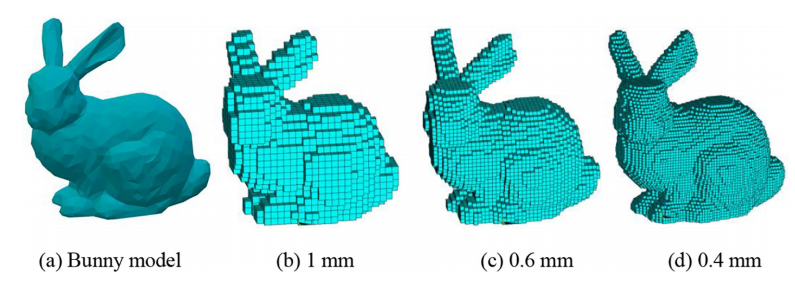
\includegraphics[width=0.7\textwidth]{images/bunny-voxelization.png}
        \caption{Bunny model voxelized at different resolution settings, taken from \cite{zhou2020voxelization}.
        }
        \label{fig:open3D-voxelization}
\end{figure}


Work on voxelized representations of the world have a number of advantages in a variety of use cases that this thesis work is inspired by and takes advantage of, such as as \cite{xie2020linking, zhou2020voxelization, dong2004real, loop2013real, orts2016holoportation}. First, they are space efficient, which makes it easier to store and use a representation of the world, and secondly, since the cubes are a finite volume, they are not restricted by the size of the camera or the resolution of the sensor. Finally, we believe that working with cubes will improve the exploration, because the representation has fewer properties and the agent has more control over the space it perceives. This final property allows the agent to be \textit{visual-agnostic} in the navigation task and understand any kind of environment regardless of the underlying data distribution. This represents a potential bridge for transfer learning tasks for navigation, where the data distribution and preprocessing steps play a critical role in the performance of an algorithm.


In this work, we use an underlying version of a voxelized world, with an isometric representation. The main idea behind voxelization is to represent the world into a medium-sized set of cubes, each representing a specific volume. Each cube can be perceived by the agent and scanned, which awards the agent reward $R^{VOX}$.
% is the first type of reward for our agent. 
There are many methods for efficient voxelization of an environment, as seen in \cite{dong2004real, loop2013real, orts2016holoportation}. For more information on the voxelization process, please refer to Appendix \ref{appendix:unity3d-voxelizing-3dmodels}, which includes the script used to pre-generate a voxelized representation of the 3D assets in the environment.


% \subsection{grid sensors: Vision in the Learning Agent}
\subsection{Grid sensors and Vision from Monocular Cameras}\label{chap:3:gridsensors}
On the topic of vision, panoramic cameras are currently actively used in visual SLAM research given not only their wide range of information perception but also the fast and complete acquisition of information they enable \cite{rill2021collision, wojek2012monocular}.
It is also claimed that spherical cameras will become the norm for driver assistance, traffic safety and autonomous navigation, where visual SLAM techniques must reduce uncertainty as quickly as possible in dynamic environments to prevent collisions \cite{zhang2021panoramic}.
% Recent research \cite{zhang2021panoramic} promotes the usage of monocular cameras as a cheaper alternative to the RGBD variant.



In monocular cameras, common cameras are less favored than other expensive alternatives, as they are limited to 60 degrees of view.
% Among monocular cameras, the common camera is less preferred in comparison to other, more expensive alternatives, since it is limited to an angle of view of 60 degrees and a vertical angle of view of 45 degrees.
This angle limits the amount of information input into the algorithms and adds unnecessary overheads in the extraction of features. More concretely, when the extracted feature points have a short-term duration in the field of vision, a different set of challenges and assumptions a technique must be taken, such as memory, tracking, etc. 
Accordingly, research by \textcite{davison2007monoslam} highlights that it takes less time to reduce uncertainty and correct positioning errors the longer a feature is observed continuously. For an in-depth review of visual SLAM methods using RGBD and monocular cameras, refer to \cite{taketomi2017visual, zhang2021panoramic}. 



% \begin{figure}[!ht]
%         \centering
%         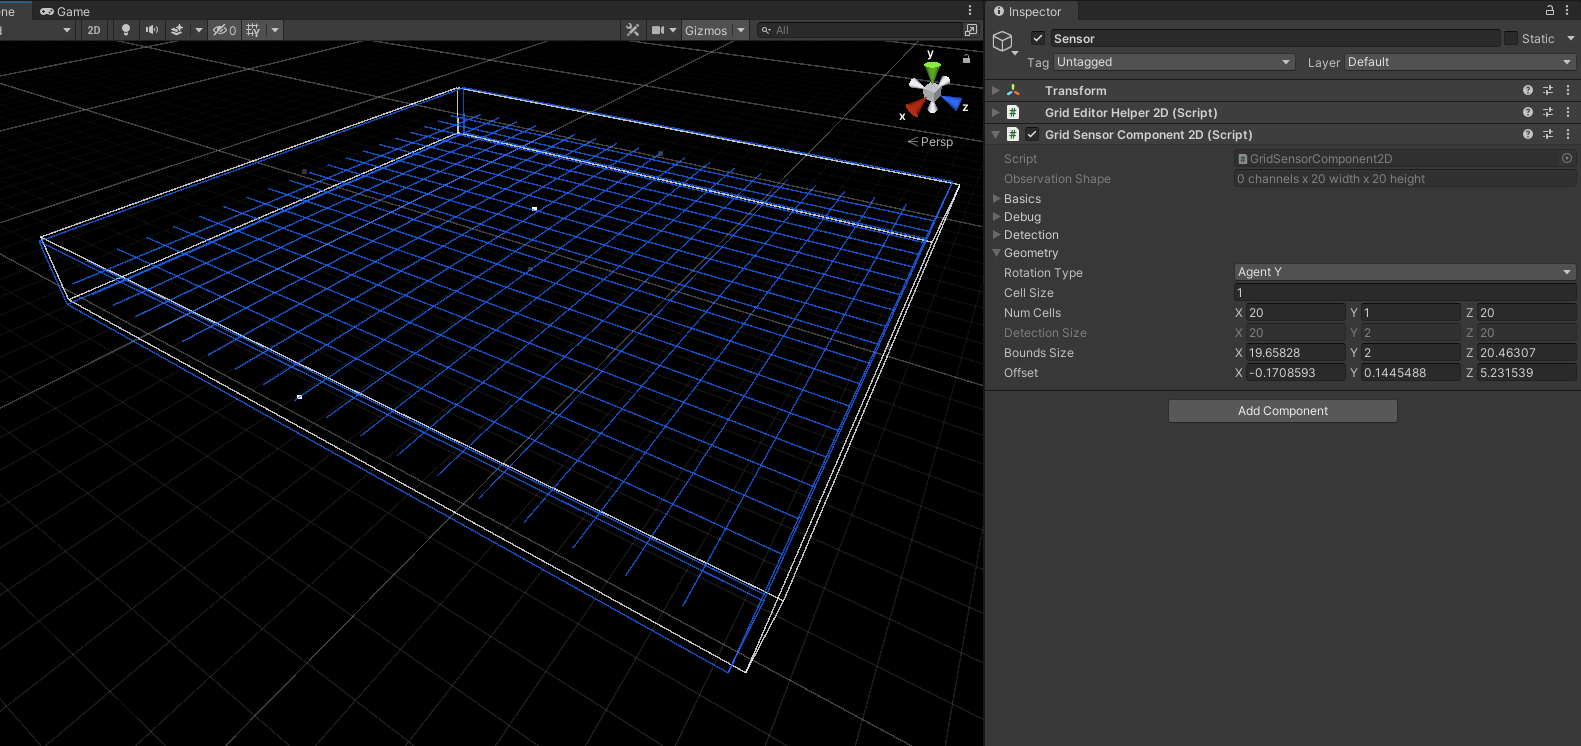
\includegraphics[width=0.8\textwidth]{images/gridsensor-scene-2d.png}
%         \caption{grid sensor 2D \cite{}
%         }
%         \label{fig:gridsensor-2d}
% \end{figure}

% Finally, recent research proves that techniques based on spherical monocular cameras perform better than their limited ordinary variant. 

% Work by \textcite{zhang2021panoramic} provides a thorough explanation of the potential of monocular cameras for the future computer vision research, where SLAM technologies are categorized into LIDAR SLAM and visual SLAM. Even though the LIDAR SLAM has been extensively studied, it remains a more expensive alternative and has a limited range of detection in comparison to camera-based SLAM. As of today, techniques for visual SLAM have used either 1) depth-sensor equipped cameras (RGBD) or 2) monocular, stereo or panoramic cameras. 

% visual SLAM algorithms: a survey from 2010 to 2016
This thesis takes inspiration from these works and the benefits provided by spherical vision, to integrate the agent with a grid sensor component.
% The motivation for the use of this component roots back to the origins of this component in the reinforcement learning community. 
The motivation for the use of this component roots back to its origins in the reinforcement learning community. 

With the growing interest for reinforcement learning techniques and research, a middle ground was required between model expensiveness and lengthy training times. Moreover, the testing of this middle ground had to be independent of the changing visuals across diverse video games, defined by one of the core principles of Automated Game Testing \cite{unity-eidosmontreal2020}. 
In 2020, the labs at Eidos-Montréal \cite{unity-eidosmontreal2020} innovated the state-of-the-art in perception for reinforcement learning, which at that point was limited to raycasts and cameras, with a simple 2D \textit{grid sensor} component. Inspired by the simplification of an environment in the MinAtar paper \cite{young2019minatar}, the grid sensor exploits the computational efficiency of CNNs with the generality in data structure provided by raycasts. The basic principle behind the grid sensor is to use a height x width x channel matrix of variable resolution, that queries physics information from objects in range. This keeps the spatial structure perceived and can be then fed to a CNN, a reinforcement learning algorithm, or used to perform data analysis. 

% \begin{figure}[!ht]
%         \centering
%         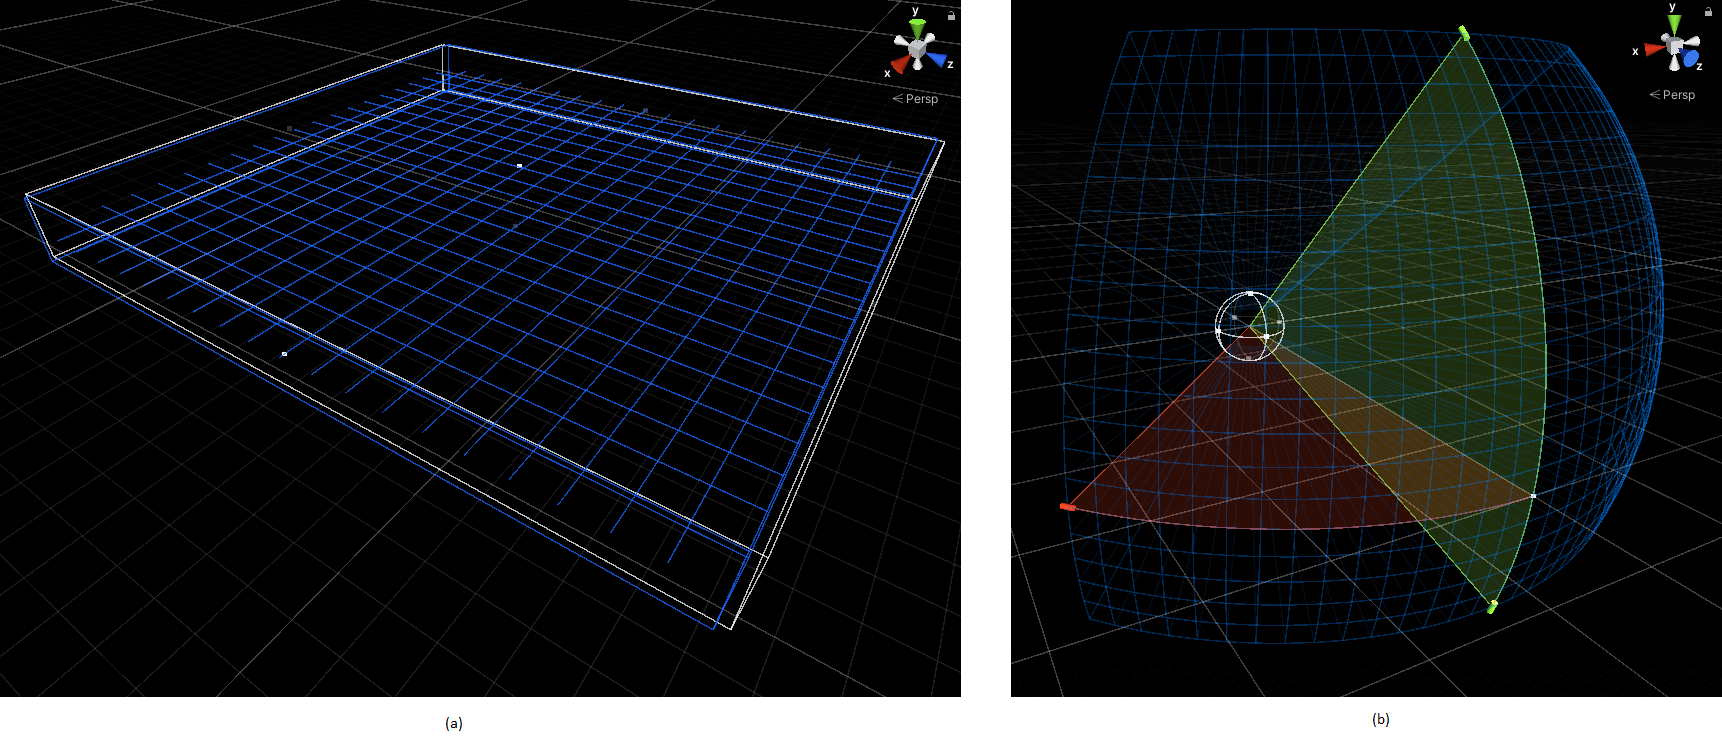
\includegraphics[width=.8\textwidth]{images/gridsensors.png}
%         \caption{Top-down 2D vision and panoramic vision through variants of the grid sensor component for Unity ML-Agents. 2D grid sensor (a) and 3D grid sensor(b), developed by Mbaske \cite{github-mbaske-gridsensor}.
%         }
%         \label{fig:gridsensor-3d}
% \end{figure}


\begin{figure}[!ht]
    \centering
    % \subfigure[]{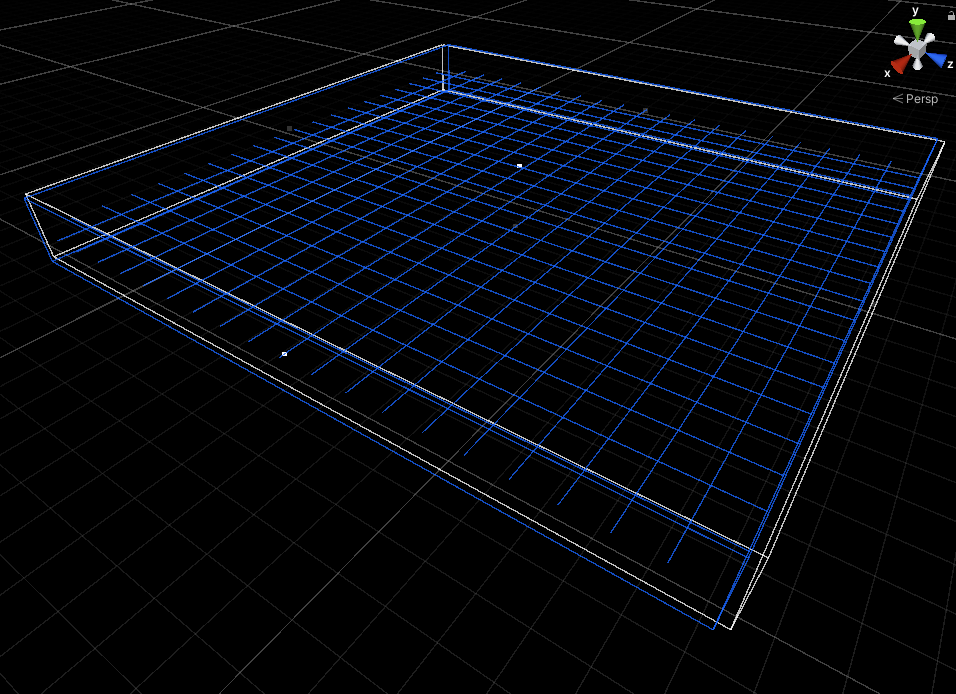
\includegraphics[width=0.538\textwidth]{images/gridsensor_mbaske_2D.png}} 
    \subfigure[]{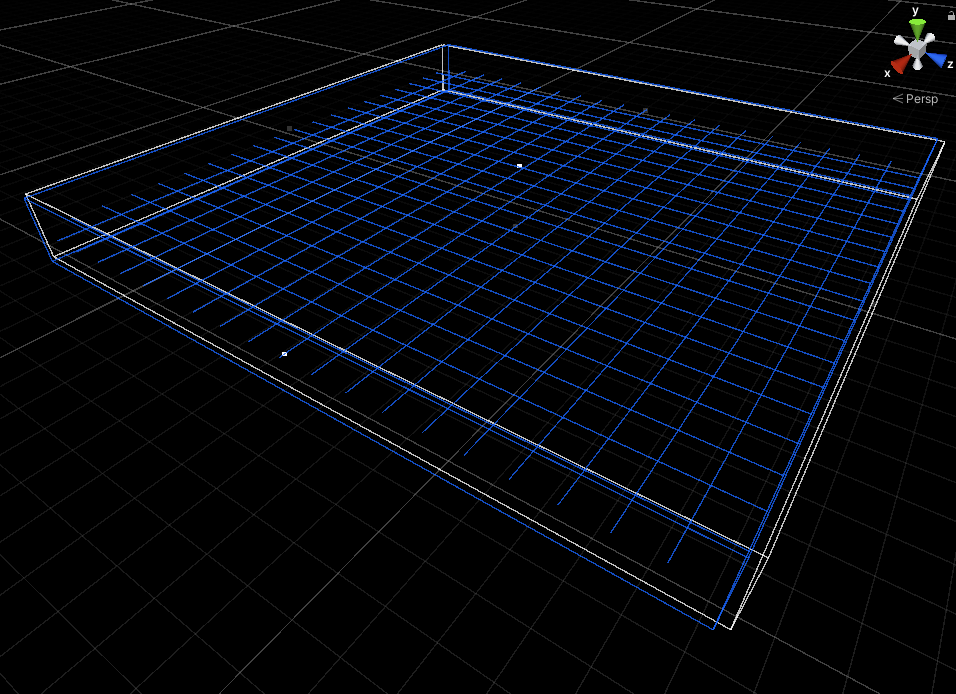
\includegraphics[width=0.4304\textwidth]{images/gridsensor_mbaske_2D.png}} 
    % \subfigure[]{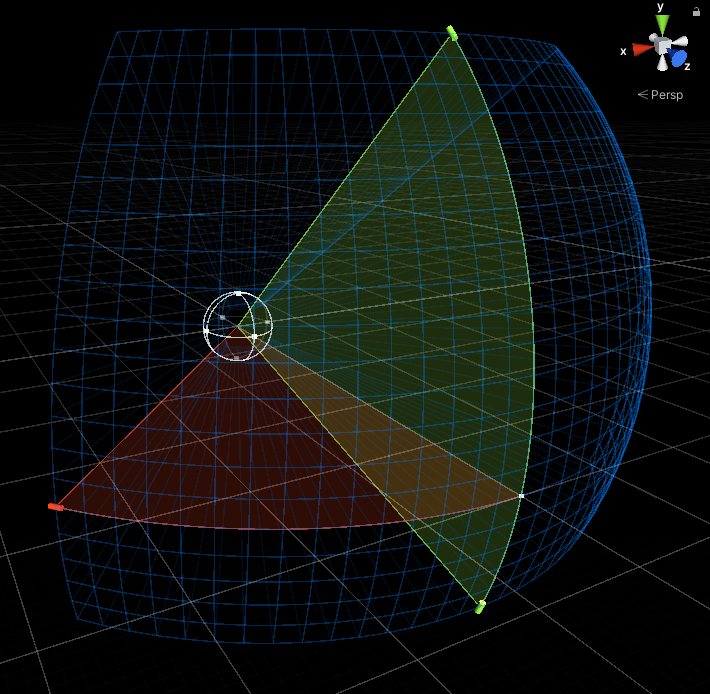
\includegraphics[width=0.40\textwidth]{images/gridsensor_mbaske_3D.png}} 
    \subfigure[]{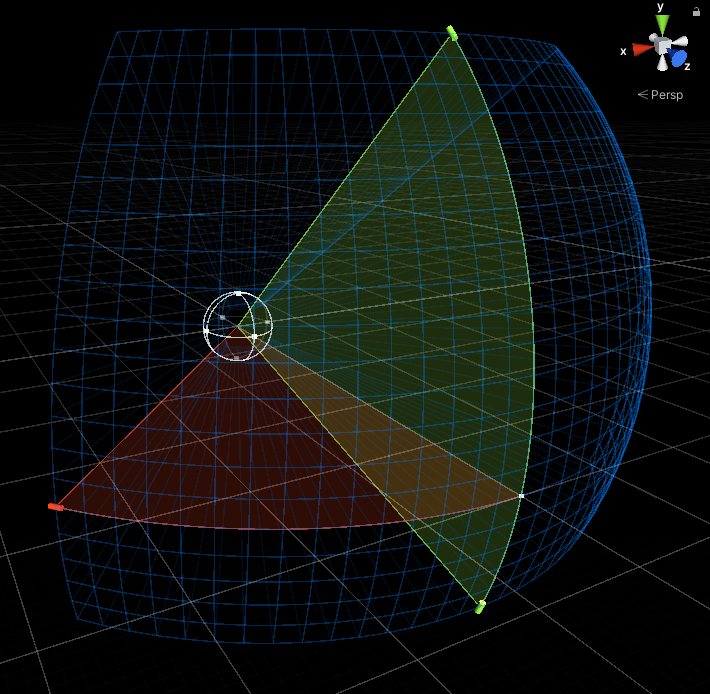
\includegraphics[width=0.32\textwidth]{images/gridsensor_mbaske_3D.png}} 
        \caption{
            Top-down 2D vision and panoramic vision through variants of the grid sensor component for Unity ML-Agents. (a) 2D grid sensor and (b) 3D grid sensor, developed by Mbaske \cite{github-mbaske-gridsensor}.
        }
        \label{fig:gridsensor-3d}
\end{figure}

The grid sensor used in this thesis is an improved version of the original grid sensor, developed by \textcite{github-mbaske-gridsensor}, under a variety of perception parameters. 
In Chapter \ref{chap:4} we compare the performance of the agent under an ordinary monocular camera setting and a spherical, panoramic, setup. 
This, in conjunction with a voxelized representation of the world, conceives a training agent that is input-agnostic and can greatly increase the training time in 3D environments. 
Since this setup does not depend on the rendering of visuals, training in the configuration file can be set to headless mode, which means that it runs as a normal computer process but no GUI is shown in the computer screen. This allows the agent to train while still using high-dimensional data and the benefits of domain randomization, such as position and domain randomization. Moreover, the 3D creative process involving textures and lighting setup is completely detached from the agent's behavior training setup. 
Our aim is that this also motivates further research in reinforcement learning to enable transfer learning of agent behaviors from training in simple environments to progressively more complex ones. 
The grid sensor developed by Baske can be found at \url{https://github.com/mbaske/grid-sensor}, and is visualized in Figure \ref{fig:gridsensor-3d}. 


% . There is extensive research into LIDAR SLAM in com 
% Panoramic Visual SLAM Technology for Spherical Images
% It refers to the use of a sensor in an
% unfamiliar environment, where the data observed by the sensor are used to estimate the
% state of motion of the sensor itself, while building a map of the surrounding environment.
% SLAM technology can be divided into LiDAR SLAM and visual SLAM. For historical
% reasons, the research into LiDAR SLAM began earlier than research into visual SLAM,
% and LiDAR SLAM technology is more mature than visual SLAM technology in theory,
% algorithms, and landing products. However, LiDAR is more expensive than cameras,
% and LiDAR has a limited range of detection. Cameras have no distance limit and cost
% less. 
% At present, the solutions for visual SLAM technology are mainly based on RGB-D
% cameras and monocular, stereo, or panoramic cameras. The biggest difference between the
% two schemes is that RGB-D cameras are equipped with depth sensors, whereas ordinary
% monocular, stereo, and panoramic cameras are not. Since RGB-D cameras are generally
% more expensive than ordinary cameras, it is of great significance to study visual SLAM
% technology based on ordinary cameras (like monocular, stereo, or panoramic cameras without depth sensors), to reduce the cost. 
% Among the ordinary cameras, panoramic cameras
% have gradually become one of the hotspots in the field of visual SLAM research because of
% their wide range of information perception and fast and complete information acquisition.

% https://link.springer.com/content/pdf/10.1007/s42979-021-00759-6.pdf
% In contrast to regular cameras which can monitor one view at a time, research suggests spherical monocular cameras will become the norm in autonomous driving applications.

% \textbf{Applications of Monocular Videos.}
% Research by 

% Autonomous driving methods have shown impressive results based on monocular vision. 
% Methods calculate the time-to-collision method based on monocular depth. 
% http://stanford.edu/class/ee367/Winter2020/report/lee_hong_lee_report.pdf
% https://www.mpi-inf.mpg.de/news/spotlights/understanding-images-videos/3d-scene-understanding-from-monocular-cameras
% new

\subsection{Navigation with Octrees}
\begin{figure}[!ht]
        \centering
        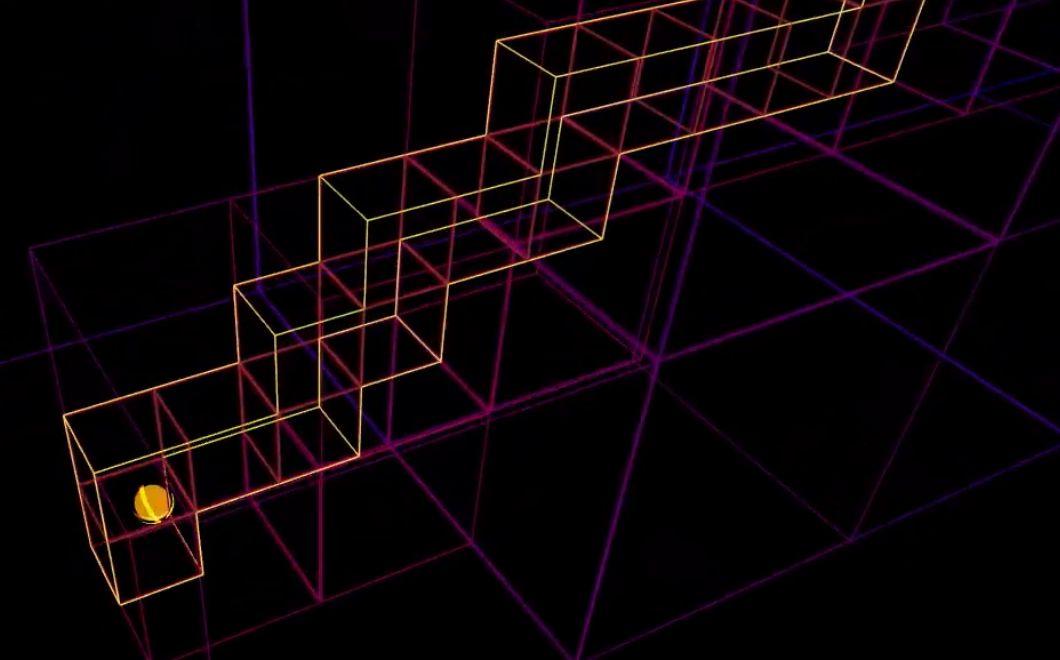
\includegraphics[width=0.5\textwidth]{images/octree-explorer-drone.png}
        \caption{Octree Construction and Navigation in Mbaske's Explorer Drone \cite{github-mbaske-explorer-drone}.
        }
        \label{fig:gridsensor-3d}
\end{figure}

As described in Section \ref{chap2:octrees}, octrees can be used to subdivide a scene in hierarchical nodes, providing a  way to efficiently deal with large amounts of space. Since our application of octrees is not meant for rendering, the drawbacks of octrees in comparison to polygons can be disregarded. 
On every step, the agent adds new nodes to the octree, which can be of three types: empty nodes (scan out of range), point (scan) nodes, and nodes that have been visited.
Information about the octree is part of the agent's observations, presented in Section \ref{chap:3:agent-choice-actions}.
The reward $R^{OCT}$ is part of the reward signal the agent receives, and it is proportional to the number of new nodes added to the octree. The reward is further defined below in Section \ref{chap:3:reward-signal}.
The implementation of octrees for Unity was taken from Baske's Explorer Drone, which can be found at \cite{github-mbaske-gridsensor}.
% here: \url{https://github.com/mbaske/ml-explorer-drone/blob/master/UnityEnv/Assets/Drone/Scripts/Octree.cs}. 

% which in our setup can be leveraged to motivate agent exploration through the addition of nodes.

% The benefits of octrees are that they give us a way to efficiently deal with large
% amounts of data and that they can be used to implement ray tracing, which is
% important for many real time applications. A
% n octree consists of a data structure
% that allows us to store data in hierarchal nodes. These nodes can be described
% as cubes and spheres in 3D space or as octagons in 2D space. The basic idea behind
% an octree is to divide a given space into a set of small cells and then to build
% a data structure that allows us to efficiently access to the contents of those cells.
% Once a space has been divided

% The disadvantages of using octrees are the overhead and memory usage associated with them. A simple octree has to store for each face (not to forget the 8 corner nodes) 8 3D vector points, and this is the worst case because most faces are triangles, but not necessarily all of them. An octree can contain between 8-32 or even 64 triangles. A simple octree is also limited to 3D vector input, not 4D tensor input. The octree can be limited in other ways (for example the octree has to be static and can be very big).


% This box representation provides some advantages for many applications, as is shown in Section \ref{octree_section}. 
% There are however some trade-offs between the complexity and size of an octree compared to that of a set of polygons. 
% % (see Table \ref{octree_table}). 
% A set of polygons can represent the same area as an octree with roughly half the number of boxes, with the advantage of being simpler to create and maintain.

% The implementation of an octree in a graphics application is beyond the scope of this paper, however there are several resources available to the interested reader, including \cite{Octree}, \cite{Octree2D}, and \cite{OctreeSectional}. We use the \cite{Octree} implementation for our work in this paper.

% At the start of the exploration process, we initialize an octree and create some random objects and their bounds. We will use this tree to represent the area of the scene the agent is currently exploring, along with any objects or bounding boxes that are inside that area. After an initial exploratory action, we then explore one area at a time by selecting the nearest neighbour of the last explored area. In our implementation, we use a greedy selection procedure, where we calculate the average distance from all objects to all other objects and then select the object with the minimum average distance. The process is repeated for each of the areas on the tree.


% This section presents the chosen definition of uncertainty or uninformativeness in an environment.

% \textbf{System Entropy.}
% In physics, entropy is defined as 

% n physics, entropy is a measure of the degree of "disorder" in a physical system. It is defined by the relation between the system's energy (work) and the system's capacity for transformation (free energy, free capacity, free energy). The entropy of an isolated system never changes. 
% entropy is used to measure the uncertainty associated with the distribution of outcomes from an experiment or a random variable. 
% In information theory, inconsistency is denoted as entropy, where entropy is a function of probability distribution functions (pdf's). If P is a pdf over the random variable X, then the entropy of P is defined as:

\subsection{Semantic Entropy}\label{chap:3:semantic-entropy}
In 1997, \textcite{melamed1997measuring} defined semantic entropy as a way to measure semantic ambiguity, uninformativeness or as the inverse of semantic reliability. In this thesis, we are especially interested in the concept of entropy as the degree of randomness or disorder in an environment, in line with the definition given in information theory, which defines entropy formally as
\begin{align*}
    H(X) = - \sum_{x\in X} P(x_i) log P(x_i).
\end{align*}
where $X$ is a discrete random variable, with possible outcomes $x_i$ and $P(x_i)$ is the probability that outcome $x_i$ occurs.

Heavily inspired by recent work on exploration by \textcite{chen2019learning} and  \textcite{chaplot2020semantic}, and as part of the answer to the research questions, we leverage the concept of entropy to define the uncertainty in an environment or a 3D object. \textcite{chaplot2020semantic} utilize semantic curiosity to learn exploration trajectories based on semantic maps. These semantic maps contain information about the inconsistency provided by an object detector at position $P$, and are used as a motivation for a reinforcement learning agent to prefer states with higher entropy. In their words, "if an object is labeled with different classes as the viewport changes, it will have high temporal entropy". Similarly, this thesis constructs a short-term memory buffer that measures the temporal inconsistencies perceived by an object detector as a way to measure semantic entropy in the agents field-of-vision. This metric, in contrast to the semantic curiosity motivation, is used to influence the linger estimator in the agent. More concretely, it acts as a discount factor in the definition of the penalty given by inactivity. The definition of the reward signal is presented in Section \ref{chap:3:reward-signal} below.



% \textbf{Reliability through Object Detection.}



% The agent started at a random location in the environment and had to navigate and reach a target location by a sequence of movements. After reaching the target location, the agent continued to move in the environment until it was back at its starting location.



% Also, under the current project's conditions it is not viable to manually annotate a point cloud. 
% It is also unfeasible to load a batch of point clouds into memory for training. Given the lack of additional inputs, each entry of the data set contains:
% \begin{itemize}
%     \item RGB image of the cow teats.
%     \item Pixel-wise segmentation mask, labeling the locations of the cow teats in the RGB image.
% \end{itemize}
% The nature of the data was two fold: synthetic and realistic. The collection of the realistic data was done at a laboratory at the ZHAW. Given the limitations of the first iteration of the milking robot project, the collection of real cow images was not required. The environment setup and details of the training data collection are described in Chapter \ref{chap:evaluation}. Finally, even though the images collected from the camera could be directly used for training, the preprocessing required was the adaptation of the data set to the COCO data format. Once formatted, the neural network could be trained.

% Consequently, the collection of the synthetic data was done using Unreal Engine 4 and a plugin from NVIDIA \cite{2021ue4} called NDDS \cite{2021ndds}. Photorealistic scenes are created in Unreal Engine 4 and NDDS allows for the annotation of objects in UE4. These scenes are then exported and all the information from the objects is included in the export, such as objects, classes and 3D poses. Additionally, the export includes the respective rgb image, depth image, instance segmentations and class segmentations for the frame taken. Appendix \ref{appendix:ndds} illustrates a 3D scene and an export sample.

% Even though the implementation computer vision pipeline required to generate voxels is out of scope for this work, we describe briefly the steps required to obtain the resulting 3D representations from RGBD images in Figure X. Captured RGBD images from a camera can be transformed into point clouds using Open3D's method 



% As described in Section \ref{chap:2:segment}, object segmentation involves the pixel-wise assignment of labels in an image that belong to a specific class. The following techniques were considered suitable for this task:
% \begin{itemize}
%     \item \textbf{Recognition of Fixed Shapes} A set of features are generated from the geometric information, such as 3D points, lines or surfaces. These features are then matched to a predefined model features. If the similarity evaluation between the model and the detected features is sufficient, a frame transformation is executed to identify the pose of the detected object. This pose detection represents a hypothesis, among many other hypothesis which are generated while evaluating, for example, a point cloud. Therefore, an appropriate criteria must be used to determine if the hypothesis should be accepted or rejected (hypothesis evaluation). An alternative approach consists of single generating descriptor features from clusters generated in a scene for posterior matching.
%     \begin{description}
%     \item \textbf{Algorithm Used: } RANSAC \cite{2021scikit-ransac}.
%     \end{description}
    
%     \item \textbf{Recognition of Object Classes} An algorithm is used to recover a 3D model from the input (image or point cloud), which is then segmented and then classified. Methods like an RDF classifier or CNNs can be used for classification. Then, methods like surface-to-surface distance minimization are used to retrieve the best match. Both realistic and synthetic RGB-D data sets have been published over the past few years for training and testing RGB-D algorithms. Furthermore, it is important that these methods are able to infer the complete 3D shape from a single frame, specially for robotic tasks like grasping.
%     \begin{description}
%     \item \textbf{Algorithm Used: } DOPE \cite{tremblay2018deep}.
%     % \item \textbf{Algorithm Used: } 

%     \end{description}
    
%     \item \textbf{Feature-based Recognition} Similarly to the recognition of fixed shapes, a set of 3D descriptor features are generated from the geometric information (keypoints) and then evaluated. These descriptor features can be defined by a set of  parameters, such as point coordinates unit vector orientations, point feature histograms of the local surface properties (PFH), etc. A major advantage of these methods is that they require only a single correct feature correspondence to recognize an object.
%     \begin{description}
%     \item \textbf{Algorithm Used: } Manual Manipulation "MAV". This algorithm leverages the segmentation mask and overlays it over the depth image. Afterwards, the 2D points are proyected into 3D space and PCA is used to calculate the teat direction. Finally, the N points (averaging method) at the bottom of the teat (using the direction indicated by PCA's first component) are averaged to obtain a "teat's tip coordinates". A manual offset was added to the obtained coordinates to attempt to fix the (x,y,z) error observed.
%     \end{description}
    
% \end{itemize}

% For each of the methods described above implementations were chosen to predict based on the data sets.  It is important, during the construction and training of a classifier, to tune the parameters of each model. On one hand, for the object segmentation approach, the parameters that were tuned were the learning rate, the score threshold for prediction, the number of workers, the number of iterations, the images per batch and the batch size. On the other hand, for the pose estimation approaches many parameters were tuned, specific to the method, such as maximum number of cow teats in memory, memory tracking reset conditions, frame transformations, etc.

% There were several challenges faced during this phase. Both synthetic and realistic data sets were used for validating not only the models but also the data sets. It was observed that 1) some implementations of the segmentation network used were slower than the final implementation used and 2) the synthetic data set was too different and the reality gap could not be closed. Additionally, allocating resources in the CPU posed a problem in the diverse training and testing. This could be solved by allocating resources in a remote GPU cluster, but set different kind of limitations in the development process.  Finally, due to the fact that many algorithms were tested, the architecture's base concept was a modular design with a plug-and-play approach.

% \section{Agent Setup}
% Once the 3D environment is constructed, the next step is to layout the capabilities of the agent. This section describes the 

\section{Specification of the Agent Character}

% The next step is the modelling and simulation of the learning agent. 
An agent is simulated through 3D assets, observations collected from an environment, actions, movement algorithms and a policy that motivates a specific behavior. The following sections provide insight into these key areas.
Furthermore, our proposal agent behavior the exploration task, is the result of a hierarchical composition of behaviors, as illustrated in Figure \ref{fig:baselines_hierarchical}. This composition starts with a base DroneAgent, that sets the basic requirements for any other agent, which includes movement, sensing and interaction. Posterior layers provide additional logic to train specific policies. For example, the \textit{SpeedDrone} takes into account variables such as angular speed, forward velocity, etc., to train an agent to  minimize the speed error between its current speed and a target speed. The same logic follows for other agents such as the OctreeAgent, VoxelAgent, ShortestPathAgent, etc., where observations that belong to the specific domain of the policy to be trained are added on top of previous layers. More detail on the hierarchical construction of these agents can be found on Appendix \ref{appendix:baselines}.

\begin{figure}[!ht]
        \centering
        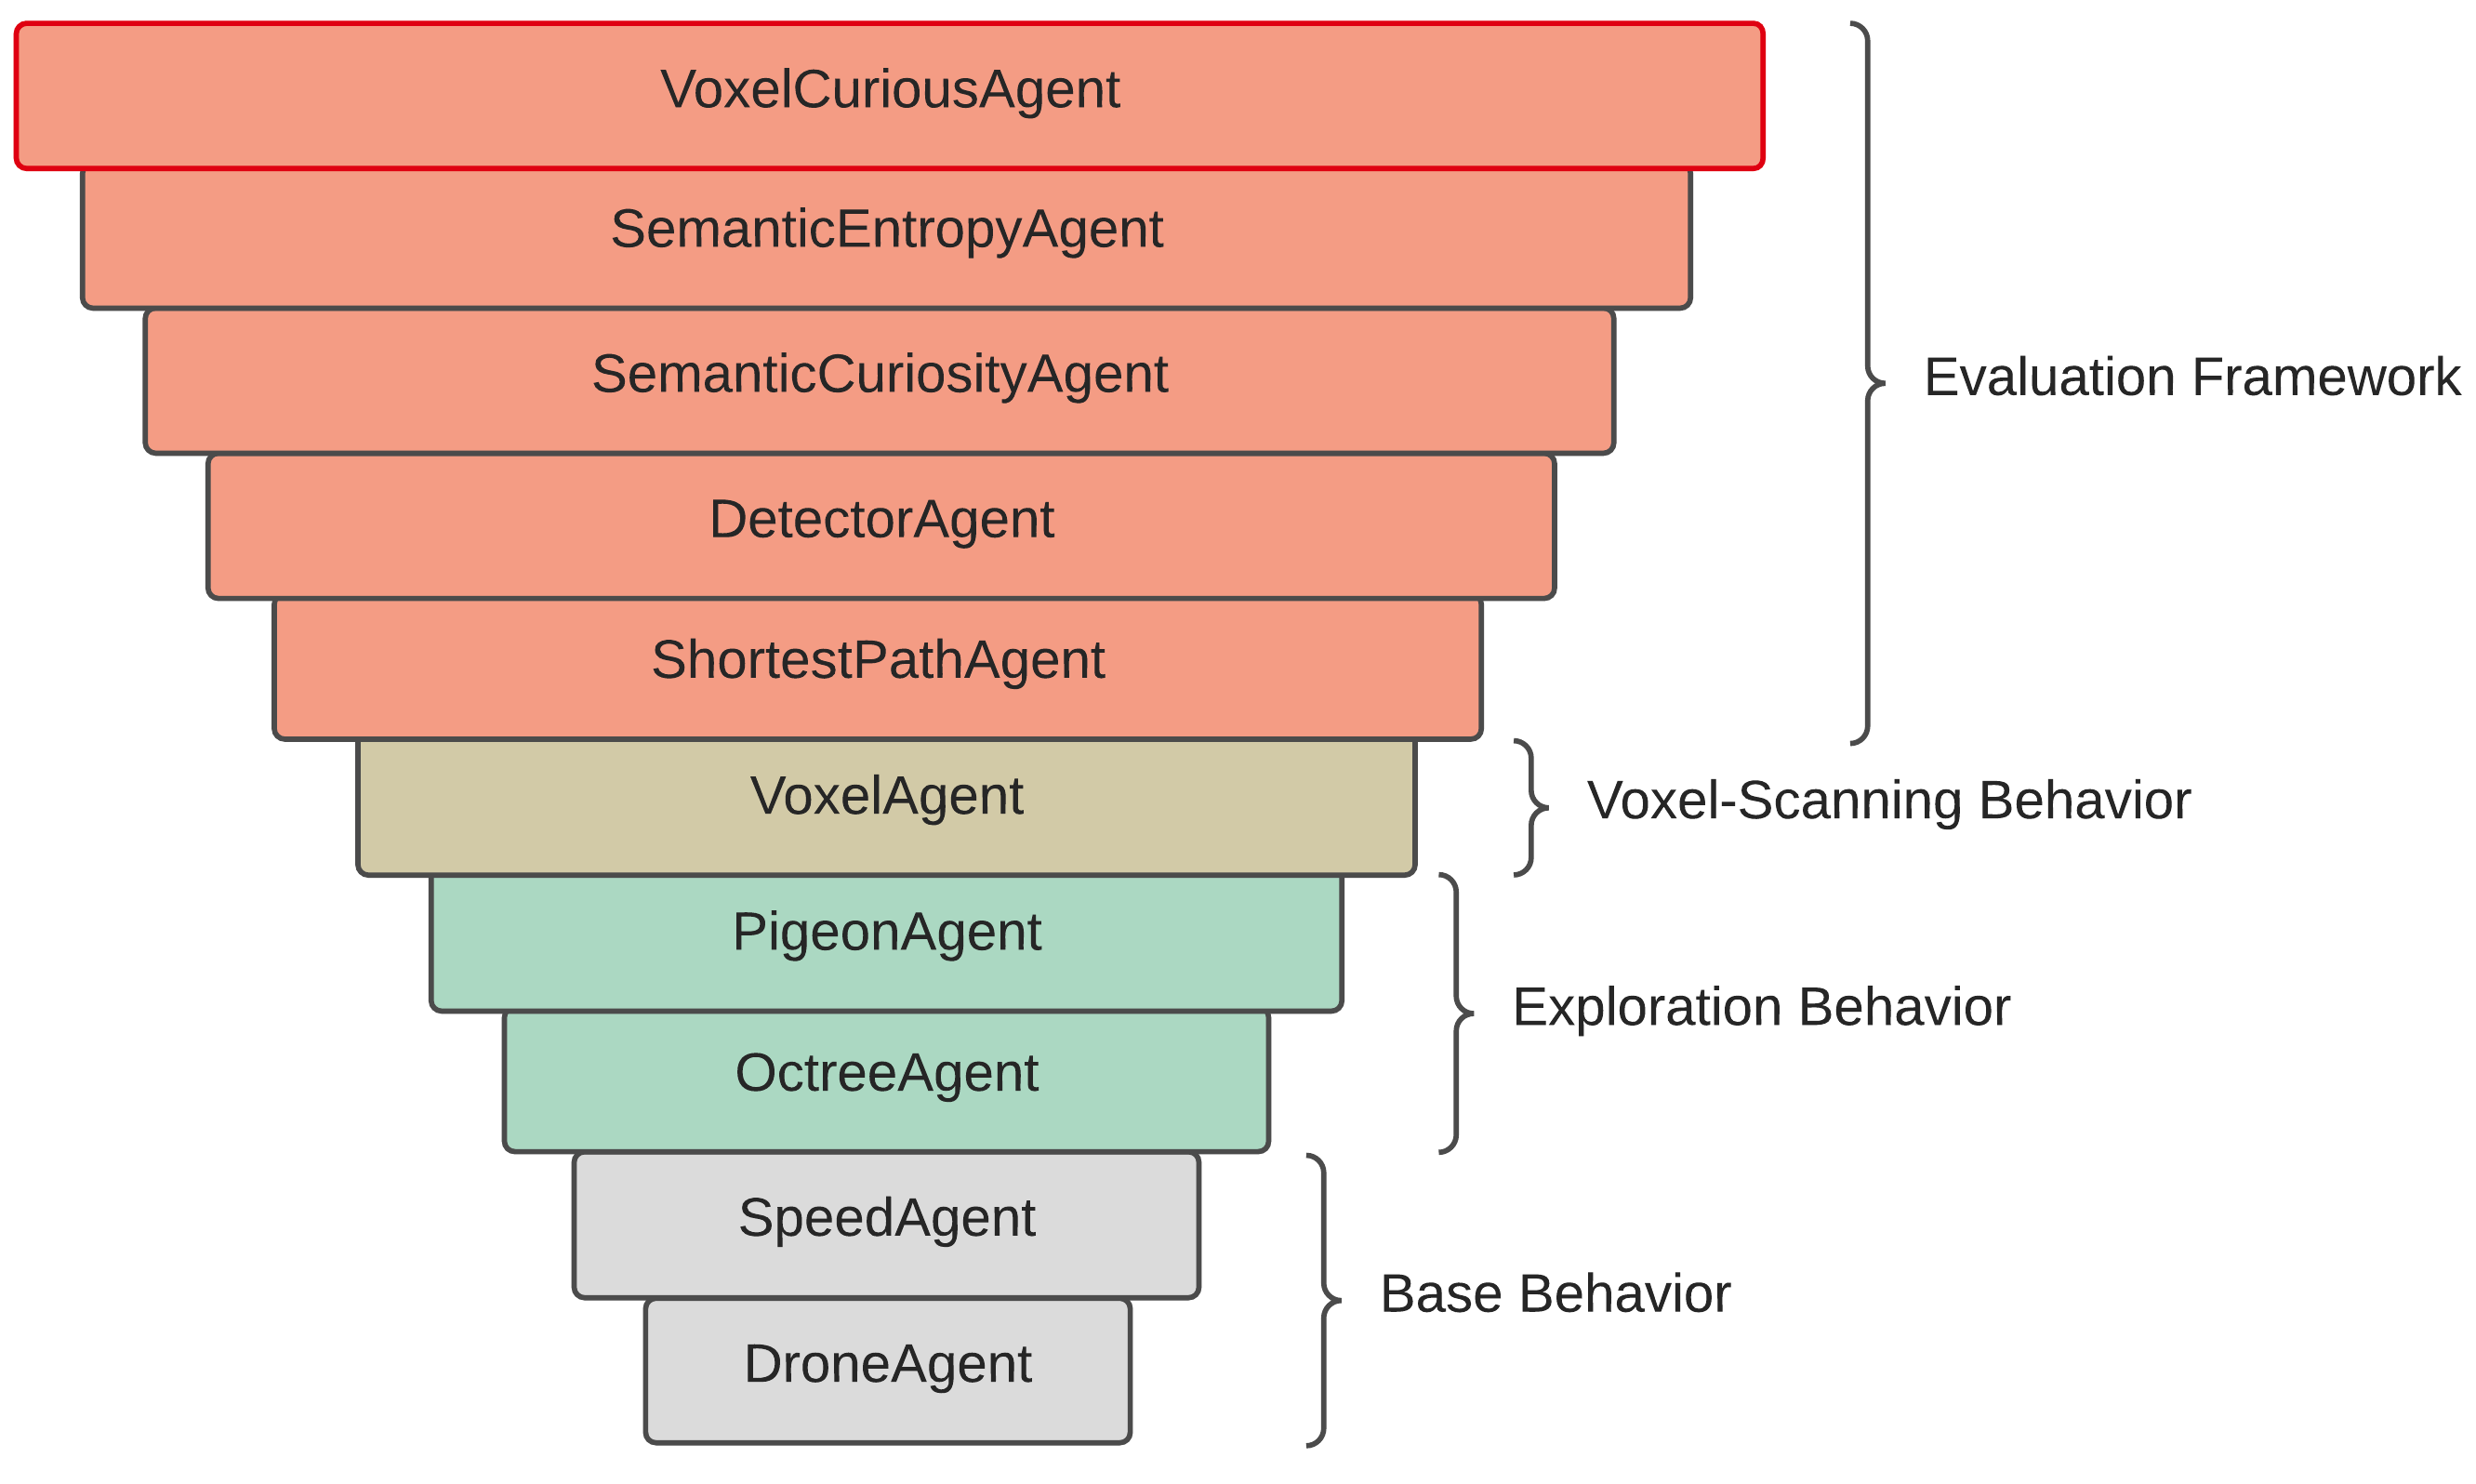
\includegraphics[width=0.7\textwidth]{images/baselines_hierarchical_construction.png}
        \caption{Hierarchical construction of the agent behaviors in Unity. The DroneAgent contains embodiment logic of the agent such as relative position and orientation. Higher behaviors inherit from the DroneAgent and implement speed, perception of octree nodes, perception of voxels, detections from a YOLO classifier, etc. 
        }
        \label{fig:bselines_hierarchical}
\end{figure}

Given that the base drone lays the ground logic for the rest of the agents, a brief explanation of its components is due. The base agent layer introduces 
\begin{itemize}
    \item A 3D model of an agent.
    \item A movement algorithm.
    \item Basic information for embodiment such as such as agent's position, rotation, its velocity, etc. 
    \item A grid sensor to enable perception of the environment, as introduced in Section \ref{chap:3:gridsensors}.  
    \item A scanner component, which enables interaction with the voxels in the environment.
    \item A reward signal.
    \item An episode reset logic.
\end{itemize}

Given that the base layer provides the foundation for other derived agent behaviors, the aformentioned elements are described in more detail in the sections below.

Similarly, the base agent allows the introduction, implementation and testing of:
 
\begin{itemize}
    \item a modeled 3D environment.
    \item an environment and goals controller. 
    \item the diverse environment platform components, described in section.
\end{itemize}
An environment and goals controller, also known as the \textit{TrainingAreaController}, looks into the randomization of the environment obstacles, goals and initializes the necessary variables for the agent’s future episode.


% % As mentioned, the base agent encompasses the necessary logic and elements required for movement, and sensing and interacting with the environment. This layer introduces the following:
% \begin{itemize}
%     \item \textbf{Basic information} is collected such as agent's position, rotation, its velocity, etc.
%     \item \textbf{Perception} is done through a grid sensor component, which was introduced in Section.
%     \item \textbf{Interaction} with the environment happens through a scanner component which allows the agent to scan voxels that fall into the constraints set, such as maximum scan distance, angle and resolution.
%     \item \textbf{Movement} is enabled thanks to a CharacterController component in two modes: translation- and physics-based. These modes are described further below.
% \end{itemize}

Consequently, composed agent behaviors follow the structure described for the base agent and incrementally add observations  and reward signals to motivate learning a different policy. In our case, the exploratory behavior is achieved thanks to the policy provided by the OctreeAgent's behavior and the policy that motivated in-depth scanning of objects is given by the VoxelAgent's behavior. More detail is provided for each derivative agent in tables \ref{appendix:baselines_observations, appendix:baselines_rewards}.


\subsubsection{3D Models}
The 3D models for the agent were obtained from the Unity Asset Store \cite{unity-asset-store} and Sketchfab \cite{sketchfab2021} as potential avatars for the learning agent in different scenarios. Figure \ref{fig:unity-drone} visualizes some models considered for the agent, where the Drone Bot was the chosen model, given the overhead complexity of animating the rigs of the other 3D models. To make the simulation more realistic, the drone was given a set of animations, volumetric lights and particle systems.

\begin{figure}[!ht]
    \centering
    \subfigure[]{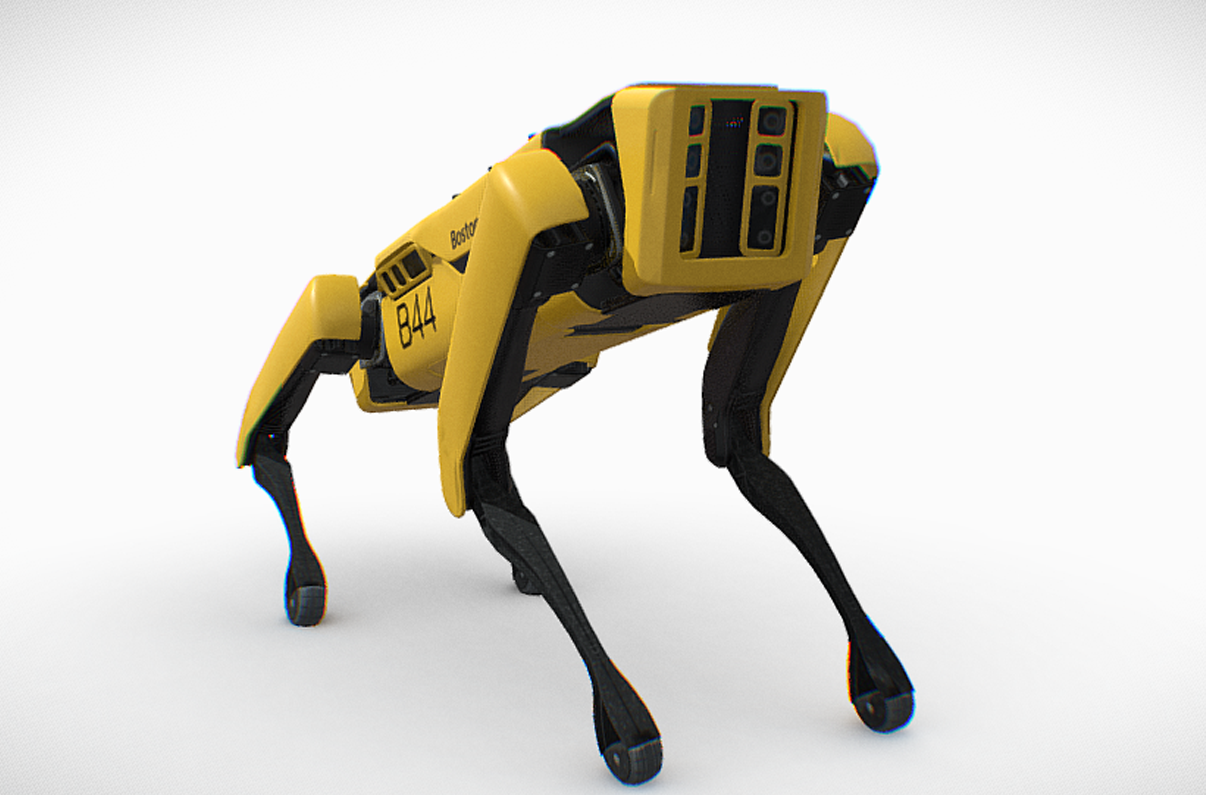
\includegraphics[width=0.24\textwidth]{images/unity-assets-spot.png}} 
    \subfigure[]{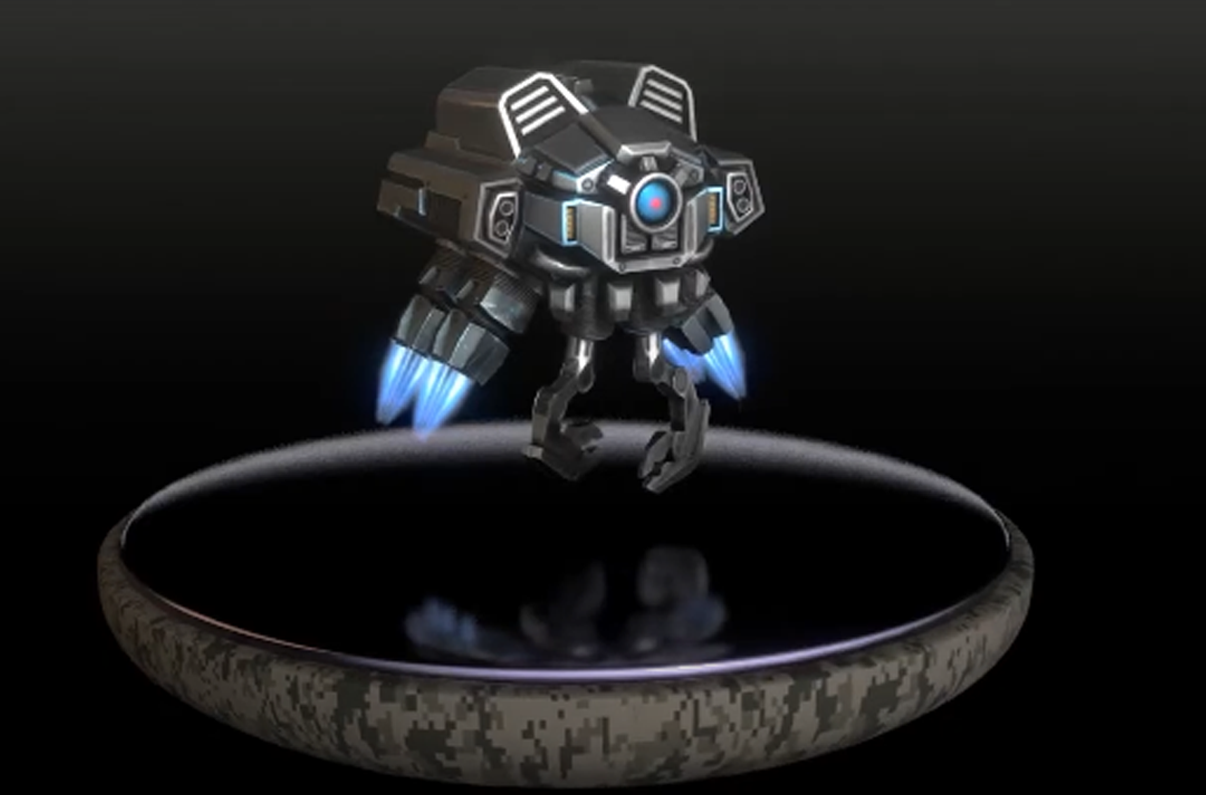
\includegraphics[width=0.24\textwidth]{images/unity-assets-dronebot.png}} 
    \subfigure[]{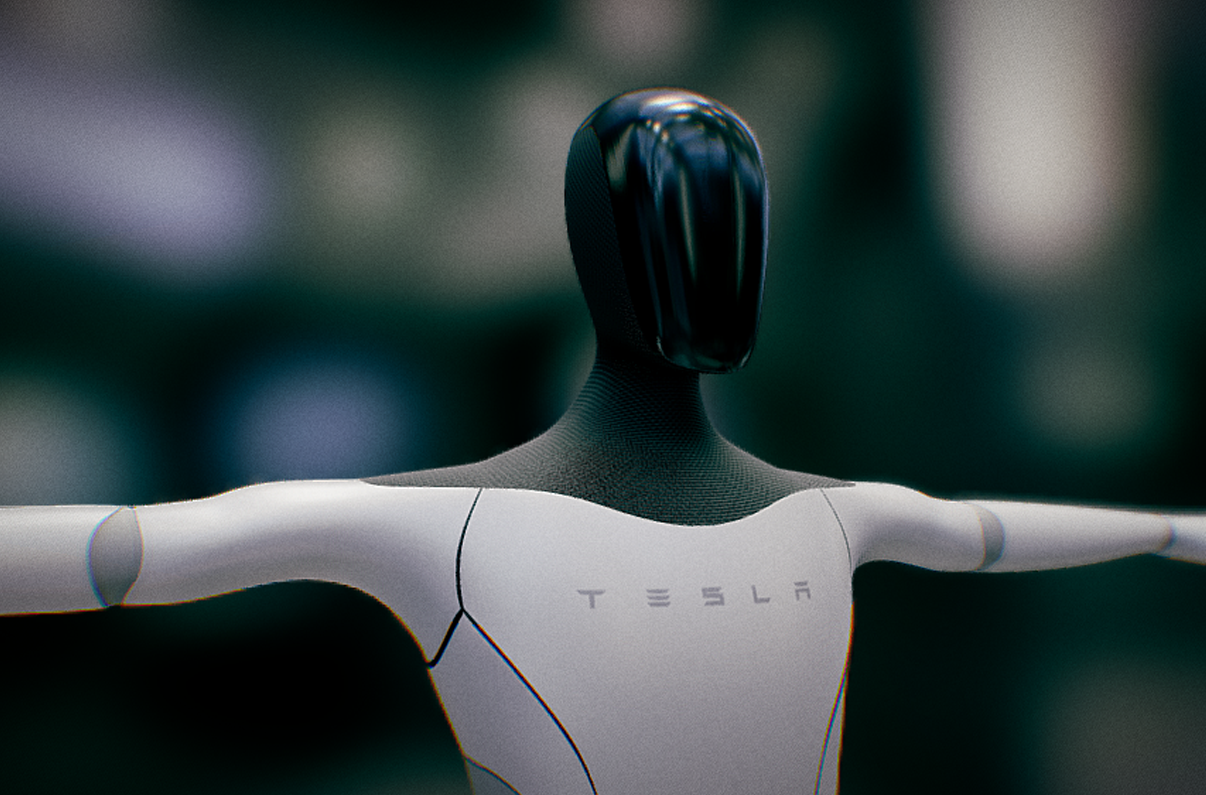
\includegraphics[width=0.24\textwidth]{images/unity-assets-teslabot.png}}
    \subfigure[]{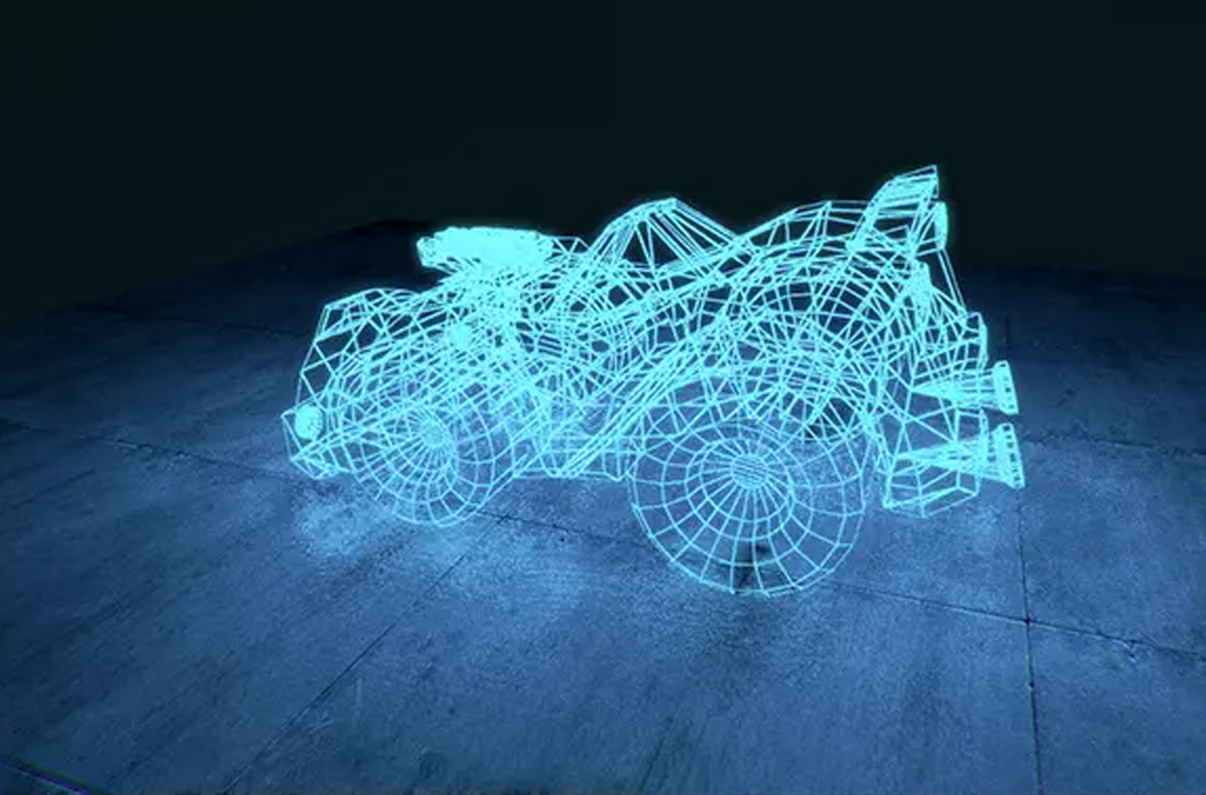
\includegraphics[width=0.24\textwidth]{images/unity-assets-wireframe.png}}
    \caption{Learning agent 3D model candidates: (a) Spot Bot, (b) Drone Bot, (c) Tesla Bot. (d) Wireframe Shader used for visualization of voxel scanning. Taken from \cite{unity-asset-store, sketchfab2021}.}
    \label{fig:unity-drone}
\end{figure}

\subsubsection{Scanner}
% affect the state of the objects around him. 
The scanner component allows the agent to scan voxels perceived from the environment given a set of constraints such as minimum angle and distance. It is made visible to a human spectator in the graphical user interface through a a special VFX feature of Unity's render engine, namely the \textit{wireframe shader} \cite{unity-asset-store}, which is displayed in Figure \ref{fig:unity-drone} (d). This shader, with the support of an invisible cone \textit{collider} \cite{unity2021} in the scanner component, modifies the render effect of the textures of objects, and displays a wireframe of the object's mesh in the intersection between the scanner's cone collider and the object's collider.

\subsubsection{Movement Algorithms}
To provide actions to the agent, i.e., to simulate a real world robot, the key challenge was the mobility algorithm for the agent. In this work, the agent was given the capability of moving in a three-dimensional environment, so it would be able of reaching any desired location.
To this end, two mobility algorithms were implemented:
\begin{itemize}
    \item Translations-based movement with a rotating function.
    \item Physics-based movement.
\end{itemize}
The simpler variant was implemented using 3D translations, applied to the agent transform's local coordinate system.
The second variant of the mobility algorithm was inspired by the movement model of a real robot, considering concepts such as velocity, torque and motor noise. Both approaches allow the robot to navigate its environment without the help of an explicit movement model.

\textbf{Physics-based movement.}
This algorithm can be defined as:
\begin{align*}
    v_t = v_t + i_t * \eta_1
\end{align*}
and
\begin{align*}
    \tau_t = \tau_t + \mu * clip(turn_t * \beta, -1, 1) * \eta_2
    % Vector3(0, 1, 0)
\end{align*}
where $v_t$ is the agent's rigidbody velocity at timestep $t$, which receives a velocity change force based on input $i_t$ at timestep $t$. This input consists of a \textit{forward input}, a \textit{vertical input}, and a \textit{lateral input}. This force is constrained by a movement speed parameter $\eta_1$, measured in meters/second. Similarly, $\tau_t$ is the rigidbody's torque at timestep $t$ which is increased by a vertical unit vector $\mu$ times the turn input $turn_t$ received at timestep $t$. The turn input is clipped to limit the possible rotation at each timestep by the agent, and is constrained by a turning speed parameter $\eta_2$.

\textbf{Translation-based movement.}
This algorithm can be defined as:
\begin{align*}
    x_t = translate(i_{xt}, i_{yt}, i_{zt}) * \eta_1
\end{align*}
and
\begin{align*}
    r_t = rotate(\mu, clip(turn_t * \beta, -1, 1) * \eta_2 * \Delta t
\end{align*}
where $x_t$ is the agent's position in the 3D space at timestep $t$, which is moved or translated based on the decomposition of the inputs received at each axis. A translation moves an object in the direction indicated by its transform's local axes. Each component from $i_t$ is previously constrained by a movement speed parameter $\eta$, measured in meters/second and regulated for smooth transitions by a time variance parameter $\Delta t$. 
Similarly, $r_t$ is the transform's rotation of the agent at timestep $t$ which is rotated by the game engine given a vertical unit vector and the turn input provided by the agent. As with the physics-based algorithm, the turn input is clipped to limit the possible rotation at each timestep. It is also constrained by a turning speed parameter $\eta_2$ and regulated by a time variance parameter $\Delta t$ to allow smooth rotations in the game engine.


\subsubsection{Additional components} 
Finally, collision parameters were also considered in the modeling of both the agent and the environment to enable the detection and avoidance of obstacles.
Therefore, the learning agent consists of the following components:
\begin{itemize}
    \item A mesh renderer that allows the visualization of the textures from the chosen 3D model.
    \item A physical body which includes a capsule collider and rigidbody components.
    \item A character controller script that captures and reacts to the input, according to the chosen mobility algorithm.
    \item An agent controller script, which is required to use the Unity \textit{ML-Agents} plugin.
\end{itemize}

The agent is therefore defined by a set of components, observations, and parameters that enable perception of both the environment and itself. 
Firstly, the components included in the agent are a 3D and a 2D grid sensor, enabling a visual input of the environment. 
Secondly, the metrics that the agent can perceive include its position, velocity, direction towards goals, etc., which register the metrics of its own rigidbody and of the objects in the environment. Finally, additional parameters such as visibility constraints, scan speed constraints and sensor noise allow the agent to learn to adapt different settings and variability configurations.
The choice of agent observations is described in the next section.
% variables that define the agent's observations can be found below in Section \ref{chap:3:agent-choice-actions}.

% are further described in the sections below. Similarly,  in sections \ref{chap:3:specification-approach} and \ref{chap:3:experiments}.




\section{Specification of the Reinforcement Learning Approach}\label{chap:3:specification-approach}

This section describes selection of a set of reinforcement learning baselines to compare our method to the choice of agent observations for the learning algorithm and the actual processing step. The following questions will be answered in this section:
\begin{itemize}
    % \item Which observations were considered for the exploration task?
    \item What reinforcement algorithm was chosen for the exploration task?
    % \item Which and how many approaches were considered appropriate for the exploration task?
    \item How was the exploration approach implemented (high-level)?
    \item What optimization steps were taken in the algorithm?
    \item What were the main problems found during this phase?
\end{itemize}

% A trade-off between machine learning techniques is always involved when comparing the advantages and disadvantages of each approach. Therefore, a variety of approaches were considered for the mentioned tasks, evaluated and optimized.


% Markov Decision Process refers to the fact that the system obeys the Markov property:
% which indicates that transitions only depend on the most recent state and action, and no
% prior history, in other words, the future is conditionally independent of the past given
% the present state. p (st+1|s1, a1, . . . ,st, at) = p (st+1|st, at)

% \subsection{Agent}


% As described in Section \ref{chap:2:segment}, object segmentation involves the pixel-wise assignment of labels in an image that belong to a specific class. The following techniques were considered suitable for this task:
% \begin{itemize}
%     \item \textbf{Random action sampling} 
%     \item \textbf{Q-learning} A K number of clusters is given to divide the data in to K groups or clusters, based on similarity.
%     \item \textbf{PPO} A histogram is used to group pixels based on gray levels, where the background is one big peak and then the other "hills" are objects.
%     \item \textbf{SAC} A histogram is used to group pixels based on gray levels, where the background is one big peak and then the other "hills" are objects.
%     \item \textbf{Curiosity} Changes in brightness are identified using filters to locate edges, curves and shapes. 
%     \item \textbf{Imitation Learning} As described in Section \ref{chap:2:segment}, convolutional operations are used to label the pixels. This approach scans the image by segments, for example using a sliding windows approach.
%     \item \textbf{Multi-Agent Environments} Contrary to to CNNs, FCNs can take different kinds of input, and output a matrix of dimensions H x W x C (image height, image width, number of classes).  
% \end{itemize}
% Among all the suitable methods tested, the segmentation problem was best tackled using two implementations of MaskRCNN: matterport/MaskRCNN and Detectron2 (FacebookAI). The evaluation and performance of both approaches is described in Section 5.

% Approaches out of scope using images are discarded given the overhead in training times given the 
% latency of images. algorithm itself would reach a similar performance just in a longer time.

% In the evaluation of the each policy, a variety set of hyper-parameters were also tested such as the extrinsic reward rate, curiosity, batch size, horizon, 

Among the multitude of reinforcement learning methods, this thesis work uses Proximal Policy Optimization (PPO), which was presented in Section \ref{chap2:ppo}. This algorithm was chosen given its demonstrated performance in a variety of tasks \cite{berner2019dota, akkaya2019solving, schulman2017proximal, yu2021surprising}, its simplicity compared to other implementations \cite{schulman2017proximal}, and general robustness. A robust algorithm shows stable performance without high dependency on hyperparameter tuning procedures or hyperparameter searches \cite{schulman2017proximal}.

The neural network used is an implementation of the original by \textcite{schulman2017proximal} taken from \cite{github-unity-mlagents-toolkit}, and it is composed of two hidden layers where the number of hidden units is part of the hyperparameter tuning process. 
This network was chosen given its demonstrated performance in \cite{mnih2015human, kempka2016vizdoom, lample2017playing}, sample efficiency in comparison with other off-policy methods \cite{yu2021surprising}, and the added benefit that its reduced size allows faster training times.
PPO requires the approximation of both the state-value function and the policy, which can be done with a shared-parameter network with two heads or two separate networks. We have opted for a shared-parameter network as in the original work by \cite{schulman2017proximal}. 

\begin{figure}[!ht]
        \centering
        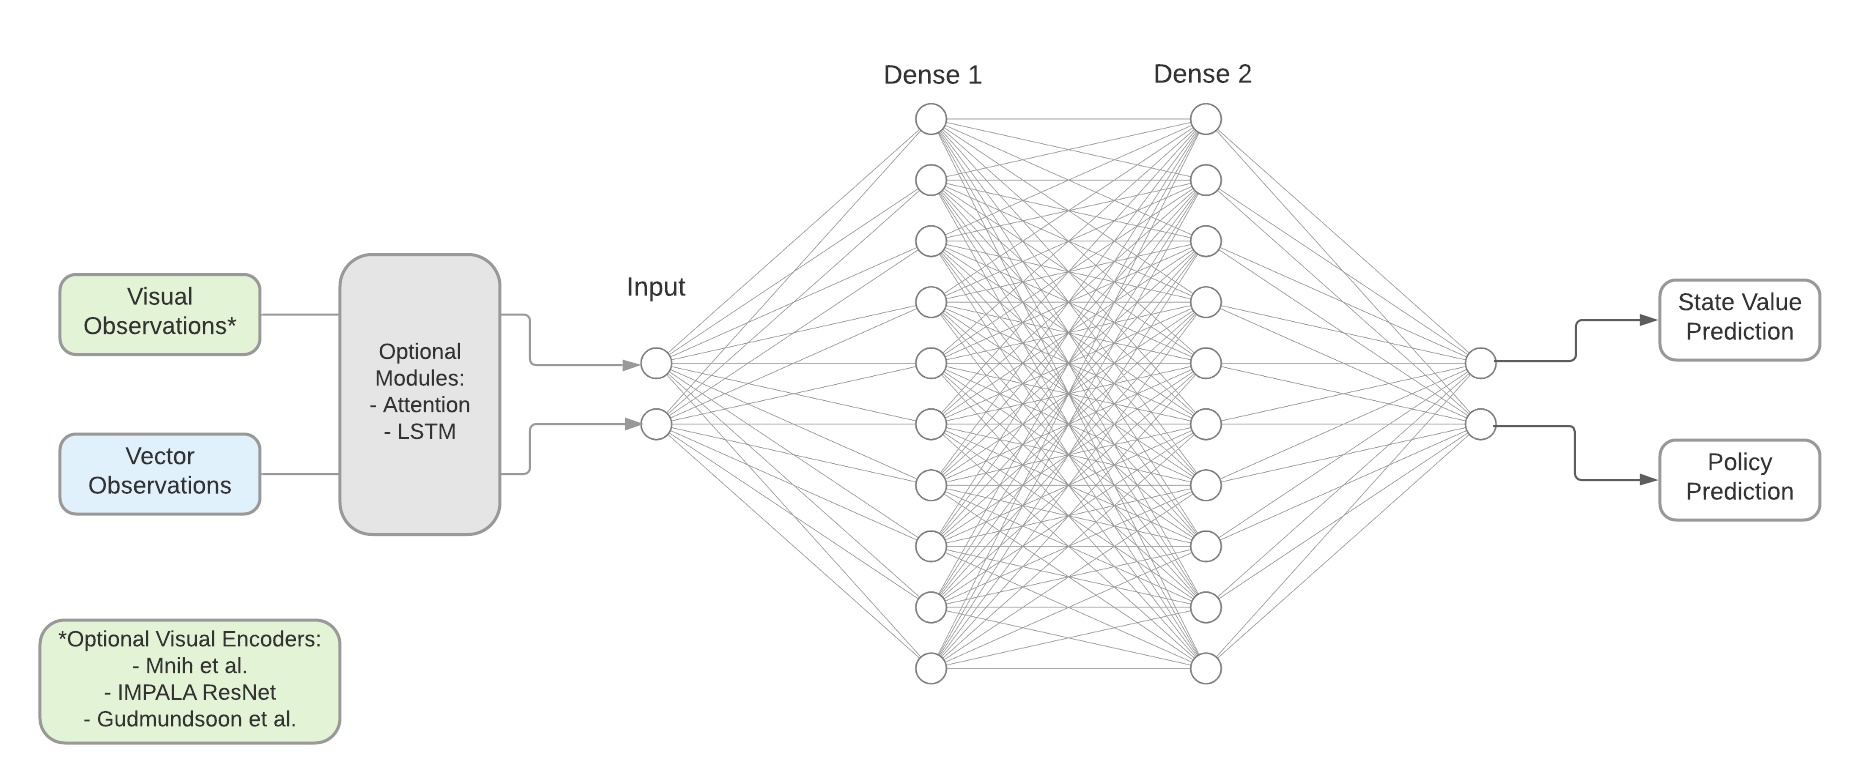
\includegraphics[width=1\textwidth]{images/PPO-unity (1).png}
        \caption{Overview of the PPO Trainer's workflow from Unity ML-Agents. Figure adapted from \cite{github-unity-mlagents-toolkit}.
        }
        \label{fig:unity-drone}
\end{figure}

The workflow for each trainer is presented in Figure \ref{fig:unity-drone}, using Unity ML-Agents \cite{github-unity-mlagents-toolkit} as the target platform. The development of the scenes and training of the agent was performed on a Windows 11 machine with an Intel i7-8700k CPU and 32GB RAM.
% and training process 
% Figure {} presents an overview of the PPO trainer from ML-Agents. 
The trainer can receive both visual observations, such as camera, raycasts, grid sensor inputs, and vector observations. Vector observations are any attribute set to observe, such as position, velocity, number of nodes in octree. Additionally, the visual encoder that receives the visual observations can easily be swapped for one of the following: 
\begin{itemize}
    \item A simple encoder with two convolutional layers.
    \item A CNN implementation by \textcite{mnih2016asynchronous}, which contains three convolutional layers.
    \item The IMPALA ResNet \cite{espeholt2018impala}, which has three stacked layers, each with two residual blocks.
    \item The "match3" CNN by \textcite{gudmundsson2018human}.
    \item A single fully connected dense layer.
\end{itemize}

Similarly, capabilities such as attention, LSTM, curriculum learning, multi-agent setups and more can be easily changed or added in Unity to construct an agent for a variety of practical reinforcement learning scenarios \cite{github-unity-mlagents-toolkit}. Figure \ref{fig:unity-simple-encoder} presents an example of the visual encoders mentioned.
% For more information on the visual encoders, please refer to Appendix \ref{appendix:visual-encoders}.

The main challenge during this stage was the delay introduced by training a reinforcement learning algorithm, where observations are provided but the performance cannot be estimated until the agent has been trained. Hence, a method with good sample efficiency was also an important factor that was considered when PPO was chosen.


\begin{figure}[!ht]
        \centering
        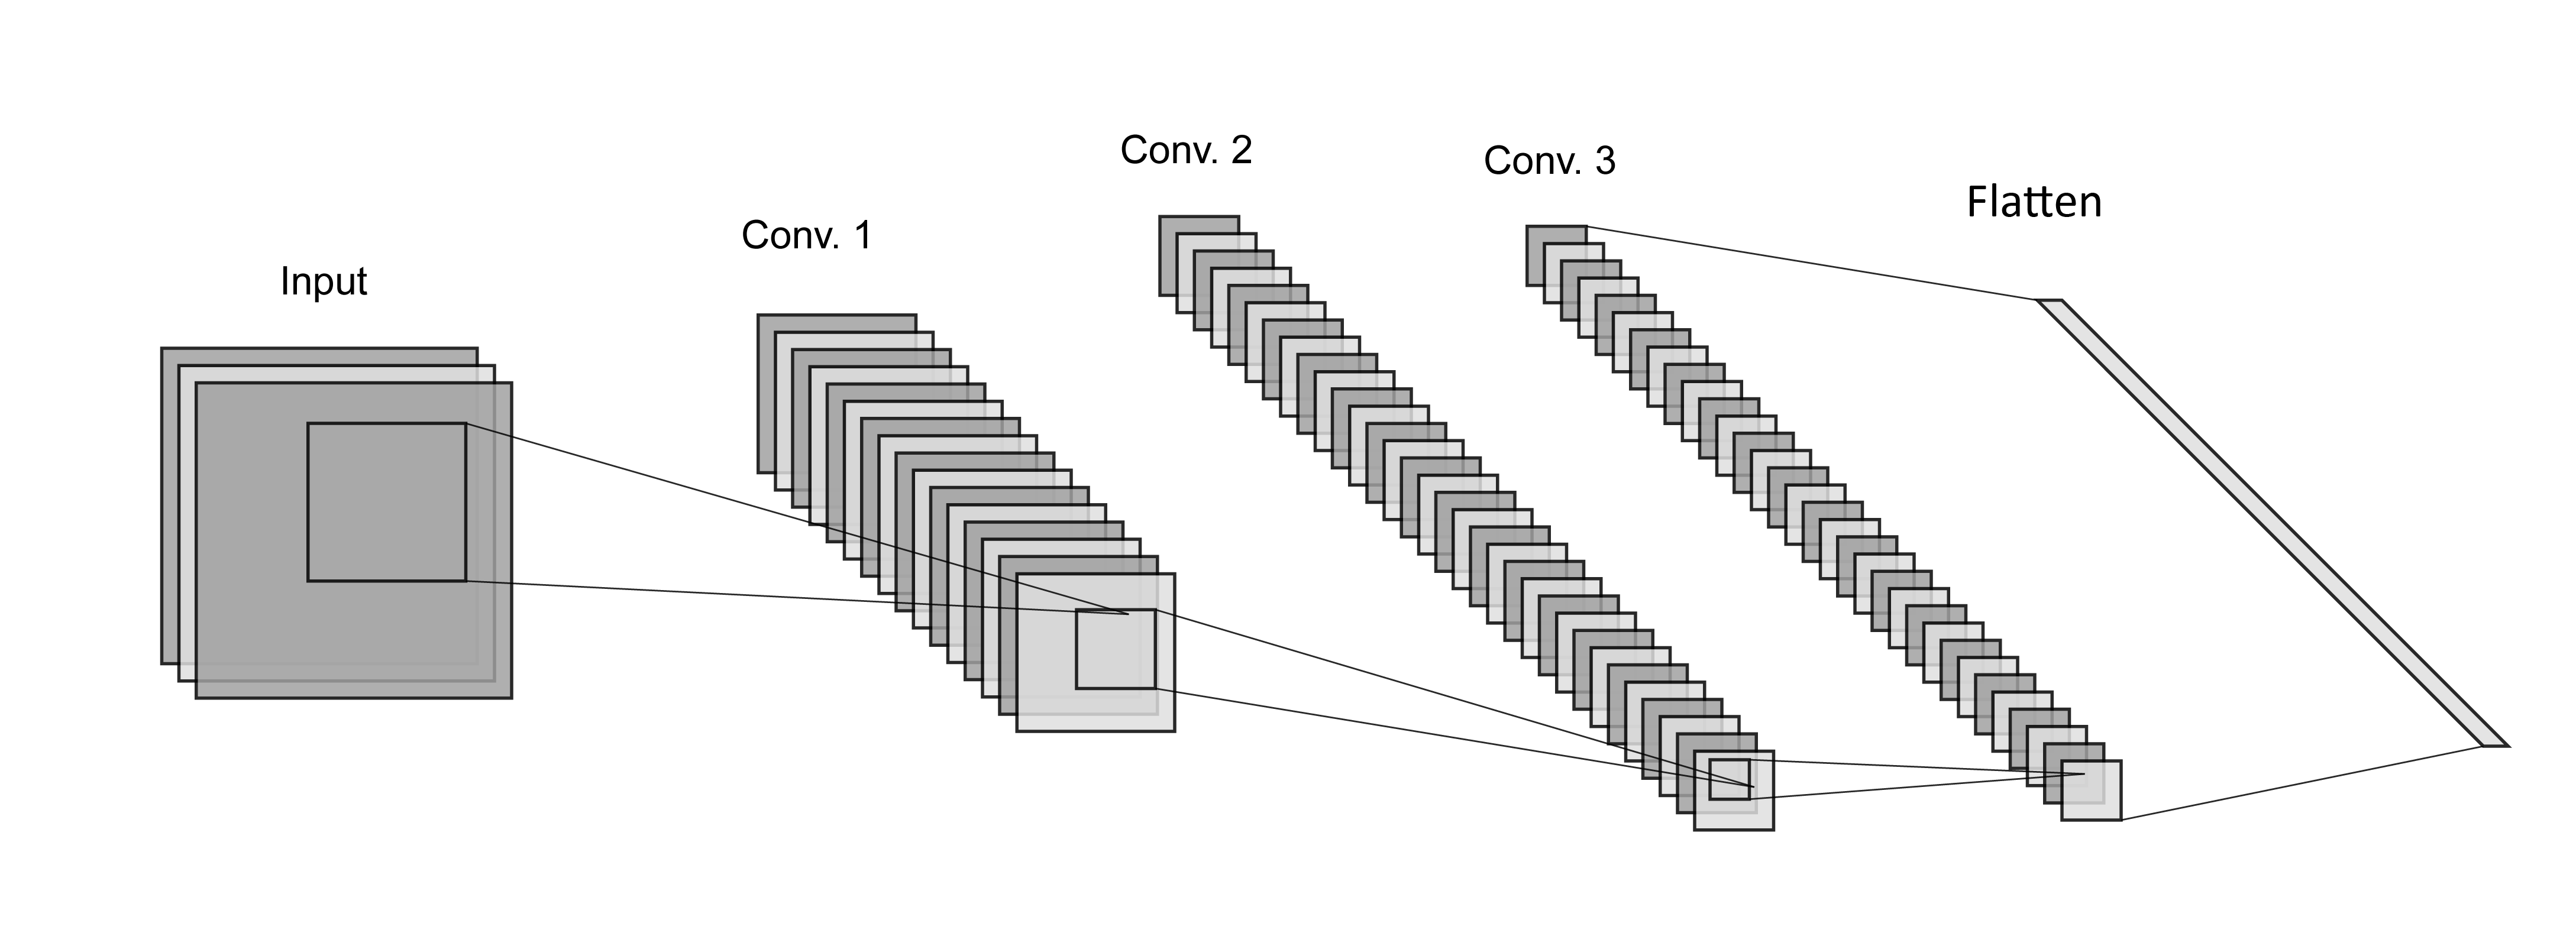
\includegraphics[width=0.8\textwidth]{images/simple_encoder.png}
        \caption{Visual encoder example, architecture by Mnih et al. Figure adapted from \cite{mnih2016asynchronous, github-unity-mlagents-toolkit}.
        }
        \label{fig:unity-simple-encoder}
\end{figure}

% \begin{longtable}{@{} p{3.5cm} p{4cm} p{4cm} @{}} \toprule
% \textbf{Layer}       & \textbf{Hidden Layer 1} & \textbf{Hidden Layer 1} \\ \midrule
% Input                &  128 & 128 \\ \cmidrule{1-2}
% Output           & An image exists. \\ 
% Activation           & An image exists. \\ 
%                         & ROSTeat node is running. \\ \cmidrule{1-2} 
% Exceptions             & Image is not RGB \\ \bottomrule
% \caption{Use Case - Predict Masks} \label{tab:use-segment} \\
% \end{longtable}





% and always converges

% This network design is quite
% small, and using a small network was a conscious choice since network size affects
% training times. 

% The network design was deemed suitable since there exists other
% image-based agents that use networks of similar size and design [10–12]. 

% In PPO,
% both the value function and policy need to be approximated, and therefore, a
% shared network was used. This means that the same base network is utilized for
% both approximations. In Tables 3.1-3.2 and Figure 3.1 the network is described
% in more detail.




\subsection{Choice of Agent Observations}\label{chap:3:agent-choice-actions}
To keep the description of the agents concise, some of the chosen observations for the agents are summarized below, without clear separations of which observation belongs to which agent. For a detailed declaration of the observations provided by each derived behavior, please refer to table \ref{appendix:baselines_observations}. This section deals with the intuition, selection, and preprocessing of observations for the learning agent. Therefore, the following questions will be addressed:
\begin{itemize}
    \item What observations were chosen for the learning agent?
    \item How do these observations contribute to the agent's learning?
    \item What were the main challenges encountered during this phase?
\end{itemize}

The selection of observations and attributes for the agent is critical for the learning method. The aim of an observation is to  represent the state $s_t$ of the environment at timestep $t$. The state $s$ is a function of a set of attributes (pixels of the image, values of variables,...) and  can be thought of as an event of the environment, where the values of these attributes have been measured.
At each step, the agent receives an observation and updates its knowledge of the environment based on it. 
Therefore, in order to learn efficiently, an observation needs to contain the right amount of information. Below are the main observations for the agent presented:

% The aim of an observation is to  provide a summary of the state, and to act as a signal for the learning rule to improve the current estimate of the state. Each observation is associated with an attribute (or a vector of attributes) that is updated according to the policy of the learning agent. The agent may observe different observations at each time step. The observations and attributes may be learned during the training phase of the agent, and are generally a function of the policy. For example, the observations and attributes may depend on the state of the agent.
% Each observation or attribute can be any numerical vector that represents the state of the agent. For example, an observation may comprise

% provide information about the environment and thus the value of taking an action. The observations may take the form of observations of attributes or observations of the environment, such as whether a door is locked or not. Each observation is associated with an observation action which can be used to take an observation of an attribute or the environment. An observation action may provide a single observation, for example the observation that a door is locked. Alternatively the action may provide a stream of observations, for example multiple observations that a door is locked over a period of time.

\begin{itemize}
    \item \textbf{Own Information}
        \\ - The agent’s position: $\mathbf{x} \in \mathbb{R}^3$.
        \\ - The agent’s orientation: $\mathbf{r} \in SO(3)$ where $\textbf{r}$ is represented through a quaternion.
        \\ - The agent's velocity: $\mathbf{v} \in \mathbb{R}^3$ based on the physics rigidbody attributes.
    % \item acceleration: $\mathbf{a} \in \mathbb{R}^3$
    
    \item \textbf{Motivation to Explore}
    \\ - An octree as a data structure for the 3D scene.
    
    \item \textbf{Perception of the Voxelized Environment | Motivation to Explore in Depth}
    \\ - A 3D Grid Sensor, which provides the agent with a panoramic input view, leveraging the benefits mentioned in Section \ref{chap2:scene-understanding}. It is visualized in Figure \ref{fig:gridsensor-3d}.
    % \\ - A 2D Grid Sensor, which provides the agent with information about the surroundings, i.e., distance to object colliders. 
    % It is visualized by Figure \ref{fig:gridsensor-2d}.

    
    \item \textbf{An Inactivity Metric}
    \\ - A linger parameter, which measures the slowness of the agent while staying in one place, given its velocity.
    
    \item \textbf{General Information about Targets perceived through the Grid Sensor}
    \\ - An \textit{orientation vector}, directed towards targets in view.
    \\ - A distance vector to targets in view.

\end{itemize}

Additional attributes that compose the agent class, which are not observations include:
\begin{itemize}
    \item \textbf{Attributes related to the scanner }
    \\ - The scanner component that scans voxels given the scan constraint variables.
    % , how far ahead can the agent scan voxels.
    \\ - A scan accuracy parameter to simulate noise in the scanner.
    \\ - A scan reload time to limit the speed of the scanner.
    \\ - A scan range constraint.
    \\ - A scan angle constraint.
    \item \textbf{Attributes related to the Grid Sensors}
    \\ - A visibility range constraint for the objects seen by the 3D grid sensor component. This variable also intervenes in the addition of empty points to the octree
    \\ - A visibility angle constraint for the objects seen by the 3D grid sensor component.
    \item \textbf{Attributes related to Mobility}
    \\ - A parameter to specify the mobility algorithm. % \textit{steuernmodus}.

\end{itemize}


One of the main problems that was encountered during this phase was finding the appropriate attributes that provide enough information to the agent about its environment while also tackling the challenge of exploration based on a different kind of input (voxels). 
A decisive factor to choosing this approach were the direct benefits obtained through the components and the nature of the approach. The understanding of a voxelized world abstracts the environment from the drone's perspective and makes its behavior visual-agnostic. 
Similarly, the grid sensors outperform both raycasts and cameras in the completeness of the information perceived and in drastic reductions of computation, memory and training costs, respectively. 
As mentioned in Section \ref{chap:3:gridsensors}, another benefit acquired from using grid sensors is that the training environment can be executed in headless mode to relieve rendering bottlenecks. 
The remaining observations motivate the agent to behave differently according to different alternative secondary rewards provided, such as the minimum movement speed or a moving forward reward. These differences in behavior are further discussed in Section \ref{chap:discussion}.

% This leaves the part of the research question of exploration policies with two types of problems to address:
% \begin{itemize}
%     \item 
% \end{itemize}



% \subsection{Environment}

\subsection{Resetting the Environment}
In our setup, an episode can reach its end when one of three conditions are met: a) the agent scanned all voxels in the scene, b) the maximum steps were reached, and the agent ran out of time or c) the agent collided with an object, which earns a negative reward. Once one of these conditions is met, the environment resets, which randomizes the positions and orientations of all 3D assets in the scene. This includes the agent and all goals.

\subsection{Goal and Reward Signal} \label{chap:3:reward-signal}
Given the presented concepts of voxelization, octree navigation, and semantic entropy, the proposed agent's goal is therefore defined as
\begin{align*}
    \max R = R^{VOX} + R^{OCT} + R^{COL} + R^{LIN} + R^{X} 
\end{align*}
where $R^{VOX}$ is the reward given by the voxel scans, $R^{OCT}$ is the reward from adding new nodes to the octree and $R^{COL}$ is the penalty the agent receives when it collides with an object. Accordingly, the penalty $R^{LIN}$ is granted given a linger estimator, which is a function of the velocity of the agent and the entropy perceived by the agent. The linger estimator penalizes the agent proportionally as its velocity decreases, but this factor is reduced by the entropy captured. More concretely, 
\begin{itemize}
    \item $R^{VOX}$ is initially set to 0.01 per voxel that is scanned by the agent. A voxel counts as scanned if the scanner is within the constraints given by the scanner variables (angle, distance).
    \item $R^{OCT}$ is initially set to 0.01 per new node discovered, obtained by calculating the intersect of the current octree with the previous octree.
    \item $R^{COL}$ is initially set to -1, granted on collisions with objects or walls.
    \item $R^{LIN}$ is a linger penalty function taken adapted \cite{github-mbaske-explorer-drone}, that penalizes the agent given 
        \begin{align*}
        R^{LIN} = -r_l * (1-e) t_n
        \end{align*}
    where 
    the strength of the penalty is determined by the penalty value $r_l$, set to 0.001, and throttled by the entropy $e$. %0.001 
    Accordingly, $t_n$ is a metric for how many timesteps the agent is at a given octant in the octree. It is constrained to a value range of $[0,2]$ and 
    % and updated every frame by 
    %     \begin{align*}
    %     t_n = min(200, t_n + 1).
    %     \end{align*}
    % It 
    reset when the agent moves to a new grid. 
    \item $R^{X}$ encompasses a variety of other rewards and penalties that were tested during the development process, such a reward for moving towards a target, a timestep penalty, a reward for moving forward and a reward for moving at speed higher than a given minimum. Some of these penalties did not make it to the final iterations, for example in clear cases where the agent stopped moving. Interestingly, the moving forward reward not removed: for demonstration purposes it is more intuitive for the agent to move forward towards a target in alignment with its 3D model, instead of backwards towards a target.
\end{itemize}

The main challenge in the definition of the reward signal was the subtle balance between rewards and penalties. For example, large negative rewards could lead to unstable or a very slow learning process because they indicate an absence of positive learning experience \cite{sutton2018reinforcement}. To this end, the initial values proposed above are evaluated and criticized in Chapter \ref{chap:4}.

 It is worth mentioning that a sparse reward function, in this case, refers to the lack of instantaneous rewards or penalties given to the agent per transition; giving therefore a reward when it is actually closer to the goal. In contrast, a dense reward function provides the agent with a reward or a penalty at most of the transitions it takes. This feedback can be counterproductive since the agent could have too many distractions at each timestep. This concept will prove useful in Chapter \ref{chap:discussion}.

% while small values of reward might lead to very fast learning, which could be sub-optimal, and often requires tuning of the learning rate.


\subsection{Implementation}
To summarize, the agent is constructed of a set of actions, sensors, and a scanner component that allow him to navigate, perceive, and interact with its environment. Furthermore, the agent is rewarded through the scanning of voxels and the navigation of the environment (addition of new nodes to the octree). It also takes into account the semantic entropy in the environment to modify the linger estimator's penalty, which gives the agent the chance to scan more exhaustively. The data structures, the chosen observations provided to the agent, and the learning of an exploration policy were also covered. 
% Following sections present the implementation of the agent and the environment, the performance interpretation, and the experiments.

The environment and the agent are implemented in Unity using C\# and the Unity ML-Agents platform. 
The workflow of a training session was adapted from \cite{eriksson2021deep} and is portrayed in Algorithm \ref{alg:trainer-ppo}.

{\centering
\begin{minipage}{.8\linewidth}
    \begin{algorithm}[H]
        initialize agent and weights $\theta$\;
      
        \While{train}{
            reset environment and gather initial observation $S$;
            
            \For{time step t=0,1,..., T}{
                let agent choose action $A$ based on state $S$; \\
                update graphics engine according to action $A$; \\
                gather observation $S'$; \\
                calculate reward $R$; \\
                calculate advantage $\hat{A}_{t}$\; \\
                check if episode is \textbf{done}; \\
                $S <- S'$; \\
            }
            Update weights with PPO;
        }
        \caption{PPO Trainer Workflow} \label{alg:trainer-ppo}
    \end{algorithm}
\end{minipage}
\par
}



\section{Interpretation}\label{chap:3:interpretation}

As described in the previous sections, the agent is defined through a set of observations that allow it to perceive voxels, new octree nodes, obstacles and 3D assets in the environment and the level of semantic entropy in the environment. It is also defined through a reinforcement learning approach that given the agent's observations, maximizes the reward on a given state, to solve two main tasks:
\begin{itemize}
    \item Exploration of the Environment.
    \item Exploration of Objects (voxel-curiosity).
\end{itemize}
% \section{Performance}\label{chap:3:performance}
%  This section also describes how the method results were evaluated, how the algorithmswere compared to each other and which parameters were adjusted
For the first task, the exploration of the environment is done through the octree observations and the associated reward. The lingering penalty also plays a critical role in this behavior to prevent the agent from staying at an octree node for too long.
For the second task, the exploration of objects is done through the generation of trajectories around the objects themselves. These trajectories are discovered through the scanning of voxels i.e., the agent is capable of looking at objects from multiple perspectives given its perception of the voxels that comprise the object of interest and the reward it obtains through the scanning of such voxels. 
The training of the agents on the big environment, also known as the "open world environment", is meant to serve as a preliminary training grounds for a variety of agent behaviors analyzed. These agent behaviors can be categorized in the following:
\begin{itemize}
    \item \textbf{Object-focused:} these agents have knowledge about voxels, i.e., they are capable of seeing voxels in the grid sensor. Their goal is to maximize the amount of voxels discovered in a scene.
    \item \textbf{Environment-focused:} refers to agents that have knowledge about octrees through information about nodes, lingering status and pigeon observations. Their goal is to maximize the space covered in a scene without direct knowledge of a map structure. From the concept of "coverage maximization", it would be similar to the work by \textcite{chen2019learning}, however we do not provide the agent with a map or information about how much it has explored so far.
    % \item \textbf{Octree Exploration (Coverage Exploration).} Based on  this baseline learns to maximize the total exploration of the octree. This provides intuition about the influence of the octree for navigation of the 3D volume.
    \item \textbf{Mixed-focus: }these agents possess both knowledge about voxels and octrees, similar to the two previous agent styles. Their goal is to find a balance between exploration of the environment and of objects.
    \item \textbf{Baselines:} these agents are meant to critically evaluate our approach from a research perspective and compare the usage of voxels and octrees for exploration to other relevant efforts in the reinforcement learning for exploration research. They do not posses knowledge about voxels or octrees, in order to provide insight of the value of voxels and octrees to both research questions.
    Following the work done by \textcite{chaplot2020semantic}, the baselines considered suitable for this task are presented below and justified:
    % The baselines are the following:
        \begin{itemize}
        \item \textbf{Random Walk.} A baseline that samples an action randomly, used to evaluate both object- and environment-focused agents.
        \item \textbf{Shortest Path.} This baseline provides the agent with the look angle and the walking angle to the nearest unvisited object. It is used to evaluate both object-focused agents given its priority for objects. %  through an orientation vector and the 3D position of the voxel
        \item \textbf{Prediction Error Curiosity.} Based on the work by \textcite{pathak2017curiosity}, it provides the agent with intrinsic curiosity towards novel states. This is used to evaluate and environment-focused agents.
        \item \textbf{Object Exploration.} This is a naive baseline where the reinforcement learning algorithm maximizes the amount of object detections given by a YOLO detector. As pointed out by \textcite{chaplot2020semantic}, this policy is expected to learn to search for frames with more objects but not for frames with different objects over time.
        \item \textbf{Semantic Curiosity.} This baseline is based on the work by \textcite{chaplot2020semantic}, and uses semantic curiosity to prefer trajectories with high temporal inconsistencies in an object detector. 
    \end{itemize}
    \item \textbf{Proposed methods:} these are our proposed methods that incorporate a mixed-focused agent logic with the semantic entropy concept.
        \begin{itemize}
            \item \textbf{Semantic Entropy.} this agent works upon the \textit{Semantic Curiosity} method by \textcite{chaplot2020semantic} by using high temporal inconsistencies in the object detector translate to adjustments to the agents lingering penalty strength. This is expected to allow the agent not only to explore both environments and objects, but also to prefer states with low lingering penalty and more objects.
            \item \textbf{Semantic Entropy as an observation.} This method is similar to the previous one by providing the semantic entropy observations to the agent, but does not adjust the lingering penalty strength.
        \end{itemize}
\end{itemize}

As mentioned before, other adjustments to the agent's behavior are given such as the moving forward reward, the lingering penalty and the minimum speed penalty. Most importantly, an alternative mechanism is implemented to constrain these penalties if voxels are in field of view (FOV) of the agent, with the expectation that the agent is able to stay longer at certain octree nodes to scan objects. 

Accordingly, in order to determine if the environment or the agent required further tuning or adjustments, the average accumulated reward across all runs was the main metric to distinguish a good from a bad performance. A low or negative reward can point to a behavior that is stuck, spinning or does not explore to discover new states with higher rewards. Similarly, a high reward can indicate a good performance but also reach undesired states. For example, after scanning most of the voxels, the agent can sometimes fall into a sparse reward situation, which complicates learning \cite{sutton2018reinforcement}.
On one side, the movement speed, turning speed, and constraint attributes related to the agent's perception were observed to analyze the agent's performance. On the other side, the agent's mobility algorithm was also observed and tuned to determine the added complexity of learning a physics model through function approximation.
The interpretation of the performance was additionally evaluated through more meaningful metrics listed below metrics and visual inspection, in order to distinguish the subtle influence of different observations and rewards in the agent's behavior:
% Firstly, inspired by the DARPA subterranean challenge, below are some of the \textit{in-depth metrics} that were collected
\begin{multicols}{2}
    \begin{itemize}
        \item Moving metrics (how fast, in which direction).
        \item Total objects detected.
        \item Total voxel detected.
        \item Total octree leaf nodes discovered.
        \item Octree nodes discovery rate.
        \item Behavior of the lingering penalty
        \item Behavior of the Shannon entropy.
    \end{itemize}
\end{multicols}
% (1) earliest time the last goal was successfully scanned, averaged across all episodes; (2) earliest time the first goal was successfully scanned, averaged across all episodes; (3) lowest average time across all scan reports, averaged across all episodes. 
Consequently, at early stages of development, visual inspection allows the viewer to debug faulty behavior, such as when the agent is stuck or spinning uncontrollably. At further stages, these \textit{in-depth metrics} allow a more intricate interpretation of an agent's behavior.
The full list of \textit{in-depth metrics} is presented in the Appendix \ref{appendix:indepth-metrics}.
% In the current task the average reward signal can further be treated as a performance metric, which should be close in performance to (3) the lowest average average time. 
% The complete list of metrics evaluated is presented in Chapter \ref{chap:4} with the results of each behavior variant.
The trainer's hyperparameters that were tuned are listed in Table \ref{tab:trainer-hyperparameters}. The full list and their default values can be found in Appendix \ref{appendix:ppo-trainer}. 

\begin{longtable}{@{} p{3.5cm} p{3.5cm} p{3.5cm} @{}} \toprule
\multicolumn{3}{c}{Tuned Hyperparemeters}\\ \midrule
% \textbf{ }       & \textbf{Tuned Hyperparemeters} & \textbf{} \\ \midrule
visual encoder type         & 
number of epochs                   & 
learning rate               \\ 

batch size                  &  
max steps                   &
buffer size                 \\

time horizon                &
number of layers            &
hidden units                \\

beta                        &
lambda                      &
epsilon                     \\\bottomrule
                            % & 
% number of epochs                        & ROSTeat node is running. \\ \cmidrule{1-2} 
% Exceptions             & Image is not RGB \\ \bottomrule
\caption{Tuned hyperparameters of the PPO trainer during the training-feedback loop, taken from \cite{github-unity-mlagents-toolkit}} \label{tab:trainer-hyperparameters}
% \\
\end{longtable} 

Table \ref{appendix:baselines_rewards} summarizes the different behaviors evaluated given variations of the observations and the rewards. These multiple variants of the aforementioned baselines were further branched off test the influences of different observations and rewards, such as the influence on performance of the visibility of voxels or the strength of the voxel reward. The training agents 
% After training the baselines and proposed variants on 3D scenes, the 
results and comparisons are presented in Chapter \ref{chap:4}. 


\section{Further Use of Results}\label{chap:3:further-use}
As stated by \textcite{luckert2016using}, the last step of every knowledge discovery process is the application of the achieved results for further use. In this thesis work, this is of special importance, where the main focus was the exploration of unknown 3D environments and the actual performance of our approach compared to a set of baselines is carried out. This section introduces the baselines that were determined to evaluate our approach, the environments were the exploration policy is deemed most useful, and the utility provided by the development with ML-Agents to perform cross-environment exploration.

\subsection{Evaluation Framework}\label{chap:3:further-use:evaluation-framework}
For the evaluation of the baseline methods and the proposed methods, we constructed two variations of the open world environment. These environment serve as testing grounds for the best performing methods from the preliminary trainings. These “DARPA Unity Scenes" are identical in dimensions and modeling but they evaluate two separate behaviors. The first environment evaluates the object-exploration capabilities of the agent through a sequential three-goal setup as shown in Figure \ref{}. The DARPA subterranean challenge \cite{darpa_subterranean_challenge} inspired the concept for these environments, where the following metrics are used to evaluate the performance of the object-exploration behavior:
\begin{multicols}{2}
    \begin{itemize}
        \item Time to object$_i$.
        \item Total time to object$_i$.
        \item Seconds per meter to object$_i$.
        \item Total seconds per meter to object$_i$.
    \end{itemize}
\end{multicols}
\begin{figure}[!ht]
        \centering
        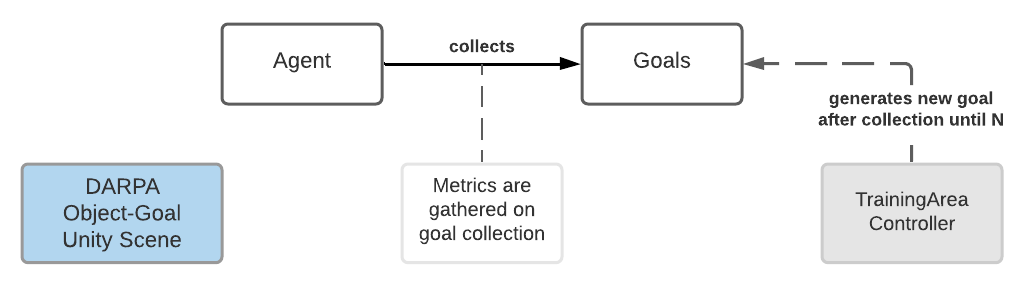
\includegraphics[width=0.9\textwidth]{images/darpa-object-setup_3.png} 
        \caption{Visual representation of the DARPA environment for the evaluation of the object-exploration capabilities of an agent in a sparse-reward setup.}
        \label{fig:darpa-object-setup}
\end{figure}
The second environment evaluates the environment exploration behavior without any goals in the scene. The metrics collected are the times to achieve 10\%, 20\,…, 90\% coverage of the scene. This is meant to demonstrate that the agent is capable of exploring multiple locations in the environment.
Consequently, the evaluation procedure is done through a bracket qualification system as shown in Figure \ref{fig:darpa-bracket}. Firstly, the best models from the preliminary training are selected. Secondly, a variable analysis is done for each of the agent behaviors: object and environment exploration. 
% This analysis as explained in section Z.
This analysis provides insight into which variables are most beneficial to the agents according to the performance observed through the \textit{in-depth} metrics. 
Finally, the qualifying runs are then evaluated on the DARPA environments where the relevant metrics for each research question are collected.
\begin{figure}[!ht]
        \centering
        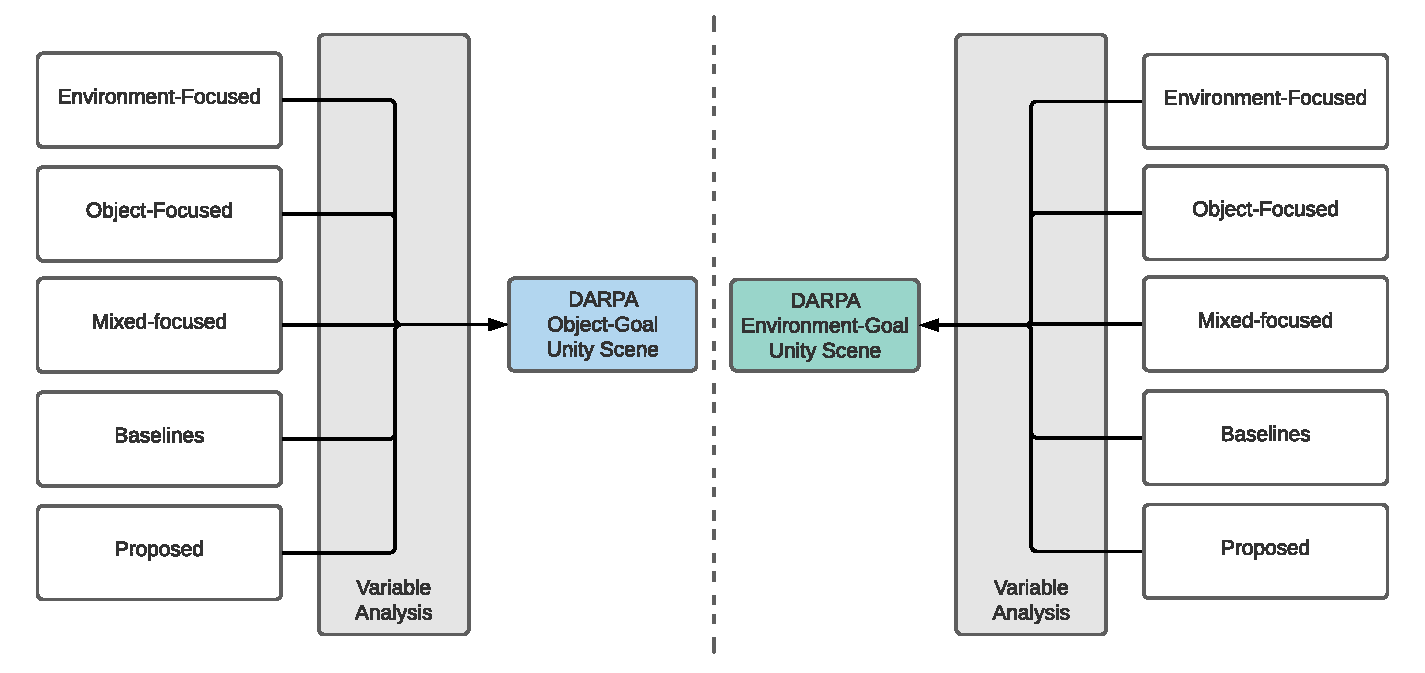
\includegraphics[width=1\textwidth]{images/darpa-qualification-bracket_2.pdf} 
        \caption{Qualification bracket system for the evaluation framework, using the DARPA-inspired testing environment.}
        \label{fig:darpa-bracket}
\end{figure}



% Figure X visualizes the bracket system as elimination rounds for the training and testing setup.


% Once the baseline methods and the

% In order to determine the actual performance of our approach, a set of metrics need to be taken into consideration to evaluate it against a set of baselines. 
% The following chapter presents a set of experiments to determine the impact of our contribution against both traditional and state of the art methods.
% performance of the different algorithms. 



% The following variants originate from our proposed method and are used to analyze the influence of different behaviors:
% \begin{itemize}
%     \item \textbf{Voxel Exploration.} This agent is motivated only through exploration of voxels. 
%     % \item \textbf{Octree/Voxel Exploration.} This is an agent which is motivated to explore not just the environment but also objects.
%     \item \textbf{Octree/Voxel/Entropy Exploration.} This agent realizes the reward signal described in Section \ref{chap:3:reward-signal}. It navigates, explores objects, and takes into account the semantic entropy in the surroundings to avoid rushing through cluttered spaces. 
%     % \item \textbf{Octree/Voxel/Entropy/BC Exploration.} This is an experimental approach that takes into account behavioral cloning. (TBD if there is enough time to include it, would add a huge bonus)
%     % \item \textbf{Octree/Voxel/Entropy/Multi-Agent Exploration.} This is an experimental approach with a multi-agent setup to observe the performance of cooperative training.
% \end{itemize}


% More detail on each experiment and metrics collected are

% \newpage
% \begin{landscape}
% \end{landscape}



% In the evaluation of each policy, hyper-parameter tuning was also explored to evaluate and compare the sensitivity of each baseline. 

% To determine the impact of our contribution we compare our approach
% %
% Among all the suitable methods tested, the segmentation problem was best tackled using two implementations of MaskRCNN: matterport/MaskRCNN and Detectron2 (FacebookAI). The evaluation and performance of both approaches is described in Section 5.

% Approaches out of scope using images are discarded given the overhead in training times given the 
% latency of images. algorithm itself would reach a similar performance just in a longer time.

% \newpage

\subsection{Usability}
\subsubsection{Applicable Practical Scenarios}\label{chap:3:further-generalization}
Part of the value behind the research questions also is reflected in the applicability of the proposed methods to a variety of scenarios. 
% The working steps to answer the research questions summarize themselves also into a policy capable of exploring any proposed 3D scene. 
Therefore, multiple scenes were considered to demonstrate the further use of the agent's behavior in production. Example scenes include a stable, a traffic accident, a neighborhood fire, a forest accident, etc.

\subsubsection{Cross-Platform Performance}\label{chap:3:further-generalization}
% In order to additionally demonstrate the value of using Unity ML-Agents
Further value of using ML-Agents can be demonstrated through the capability to transfer developed environments to another environment platform. OpenAI \cite{github-openai-gym} was chosen as the target platform, given that it is one of the go-to platform in the reinforcement learning community, with a multitude of configuration settings, algorithms, and compatibility with other frameworks \cite{github-openai-gym}.

The trainer used was the Stable Baselines 3 \cite{github-dlr-rm-baselines3} trainer, developed by the German Aerospace Center (DLR) and the Institute of Robotics and Mechatronics (RM). Accordingly, a similar average accumulated reward and a \textit{low transfer cost} across environments was treated as a high indicator for a high compatibility between environment platforms.  The transfer cost was defined as the amount of hours and lines of code required to reuse a Unity Environment in OpenAI Gym.

\subsubsection{Algorithmic Performance} \label{chap:3:algorithmic-performance}
We finally compare the performance of PPO to a state-of-the-art deep reinforcement learning algorithm, Soft Actor-Critic. 
On one hand, where vanilla RL implementations suffer from a large variance of the learned policy due to the policy update on-policy, PPO is a well-rounded algorithm that exhibits remarkable performance on a variety of tasks, as described in Sections \ref{chap2:ppo} and \ref{chap:3:specification-approach}. On the other hand, SAC is known to improve sample efficiency compared to on-policy methods and to reduce the variance through a more complex policy update (critically) and an off-policy correction step. Subsequently, SAC's off-policy training advantage is also important to analyze, because real-world problems, such as robot control, often have data from a non-replayable domain. 
% Details on the experiments carried out can be found in the next chapter.


% (write a bit more here)
% Additionally, this approach allowed 

% \subsection{Semantic Sub-modules}\label{chap:3:further-semantic}

